\documentclass[11pt,oneside]{uhthesis}
\usepackage{subfigure}
%\usepackage[margin=1in]{geometry}
\usepackage[spanish]{babel}
\usepackage[utf8]{inputenc}
\usepackage{multirow}
\usepackage{listings}
\usepackage{tcolorbox}
\usepackage{graphicx}
\usepackage{url}
\usepackage{float} %instalar manana

\graphicspath{{Graphics/}}
\newcommand{\head}[1]{\textnormal{\textbf{#1}}}
\tcbuselibrary{listingsutf8}
\newtcolorbox[auto counter, number within=section]{example}[2][]
{colback=gray!5!white,colframe=black,
fonttitle=\bfseries, title=Ejemplo~\thetcbcounter: #2,#1}
%\geometry{left=1cm}
%\geometry{right=1cm}
\newtcolorbox[auto counter, number within=section]{example2}[2][]
{colback=gray!5!white,colframe=black,
fonttitle=\bfseries}

\title{TkHURSv1.1: SOFTWARE ESTADÍSTICO PARA CALCULAR LOS PERÍODOS DE RETORNO DE HURACANES}
\author{Yasmany David Morejón Cruz}
\advisor {
Dra. Vivian Sistachs Vega
\\
MSc. Pedro Roura Pérez 
}
\degree{Licenciado en Ciencia de la Computación}
\faculty{Facultad de Matemática y Computación}
\date{La Habana, 2020}
\logo{Graphics/uhlogo}
\makenomenclature

\hyphenation{ta-re-as arro-jan na-tu-ral cons-ti-tu-yen di-fe-ren-cia pro-ble-ma pa-la-bra 
	ocu-rren-cias pro-pues-tas mo-di-fi-ca-dor va-lo-res e-le-men-to opi-nión 
	fun-da-men-tal-men-te dis-tri-bu-ir mi-ne-ría di-fe-ren-tes re-cons-truir
	dis-mi-nu-ción de-sa-rro-llan-do de-sa-rro-lla-ron
	in-fe-ren-cia po-si-ti-va es-tre-llas opi-nio-nes di-fe-ren-te pa-la-bras
	si-no-ni-mia ne-ga-ti-vo ne-ga-ti-va sub-es-pa-cio va-rian-za apro-xi-ma-da
	ejem-plos se-pa-ra-dor co-rri-das} 

\begin{document}
\frontmatter
\maketitle

\begin{dedication}

\end{dedication}
%\begin{acknowledgements}

\end{acknowledgements}
\begin{opinion}
\textbf{Opinión de los tutores del Trabajo Diploma titulado “TkHURSv1.1: SOFTWARE ESTADÍSTICO PARA CALCULAR LOS PERÍODOS DE RETORNO DE HURACANES” del estudiante Yasmany David Morejón Cruz.}\\


El trabajo de tesis desarrollado por el estudiante Yasmany David Morejón Cruz de Ciencia de la Computación aborda un tema de suma importancia como son los ciclones tropicales. La actualización el software TkHURS para el análisis de períodos de retorno a través de un Modelo de Poisson utilizando la cronología de Ciclones Tropicales en Cuba se desarrolló con el objetivo de realizar investigaciones para la prevención de estos fenómenos. Este comprende los aspectos matemáticos necesarios para realizar el análisis primario de datos que incluyan los diferentes métodos.\\


El estudiante se enfrentó al trabajo con independencia, no logró solucionar todo el problema planteado debido a los inconvenientes presentados en este período por la situación de la Covid19 y dejando claro que todas las discusiones fueron a través del teléfono fijo y WhatsApp. A pesar de todo para lograr los objetivos propuestos el estudiante necesitó hacer uso de los conocimientos recibidos en la carrera y tuvo que ver temas relacionados con la estadística y la climatología.

\begin{figure}[H]
\centering

\includegraphics[scale=0.6]{firmas_tutores}
\end{figure}


\end{opinion}
\begin{abstract}

Los más grandes desastres naturales que recoge la historia de nuestro país han estado asociados a los ciclones tropicales. La gran actividad ciclónica ocurrida en los últimos años, ha centrado la atención sobre la climatología de estos, su variabilidad y su tendencia a largo plazo. Varios huracanes han ocasionado desastres de gran significación debidos, fundamentalmente, al número de personas que murieron como consecuencia del impacto de la tormenta. De acuerdo a la trayectoria revisada de huracanes que azotaron a la Isla de Cuba, se decidió hacer la actualización del software TkHURS para obtener los períodos de retorno y calcular las frecuencias estimadas a través del ajuste de un Modelo de Poisson a la variable que cuenta el número de huracanes por año que han azotado a Cuba, en el período de 1791-2018, a partir de la Cronología de los Ciclones Tropicales y los Estados Generales del Tiempo. Se actualizó la metodología permitiendo agregar las nuevas funciones del software para una mayor comprensión a la hora de su utilización. Se realizó la validación a través de la región Central en el período 1980-2018 con los huracanes intensos, donde se pudo observar que se puede esperar un huracán intenso cada 10 años. El gráfico de pastel muestra que esta región es más afectada por los de categoría SS4 con un 50\%. Además, permitirá realizar mejores investigaciones y brindar servicios a distintas instituciones para obtener beneficios económicos. 

\begin{description}
\item[Palabras claves:]{ Huracanes, Modelo de Poisson, Software, Períodos de Retorno, TkHURSv1.1}  
\end{description}

\end{abstract}
\tableofcontents
\listoffigures
\listoftables

\mainmatter
\begin{introduction}

Los más grandes desastres naturales que recoge la historia de nuestro país han estado asociados a los ciclones tropicales. Varios huracanes han ocasionado desastres de gran significación debidos, fundamentalmente al número de personas que murieron como consecuencia del impacto de la tormenta. La gran actividad ciclónica ocurrida en los últimos años, ha centrado aún más la atención sobre la climatología de los ciclones tropicales, su variabilidad y sus tendencias a largo plazo.\\ 
En el año 2000 se culminó un estudio cuyo objetivo era confeccionar una cronología de los ciclones tropicales que han afectado a Cuba, a la luz de los conocimientos actuales, que sirviera de base para actualizar los conocimientos sobre la climatología de los ciclones tropicales de Cuba, su variabilidad y los factores que la regulan. Posteriormente, se ejecutó un nuevo proyecto denominado “Climatología de los ciclones tropicales de Cuba”, el que estuvo dirigido a prolongar hacia el pasado los resultados antes alcanzados en la cronología \cite{DK4, DK5}. La misma al día de hoy abarca el periodo 1791 – 2018 para los huracanes.\\
Es necesario saber los períodos de retorno de la afectación de huracanes a cada una de las provincias, por región y en general a Cuba. También se tiene en cuenta los Resúmenes de la Temporada Ciclónica elaborados por el Centro de Pronósticos del Tiempo del Instituto de Meteorología para los años posteriores a 1998. Se tiene en cuenta la categorización con que cada huracán afectó a cada provincia, utilizando para ello la escala Saffir-Simpson. En la Tabla \ref{escala_saffir_simpson} se presenta la clasificación de los huracanes de acuerdo con la escala de Saffir – Simpson.\\ 
%En la actualidad se denomina a los huracanes de las categorías 3, 4 y 5 como “huracanes intensos”. Los huracanes de las categorías 4 y 5 pueden denominarse “como los huracanes más intensos” o de “gran intensidad”, los de categorías 2 y 3 cómo intensidad moderada y los de categoría 1 de poca intensidad.


\begin{table}
\begin{center}
\caption{Clasificación de los huracanes según la escala de Saffir – Simpson}

\begin{tabular}{| c | c | c |} 
\hline
Categoría & Viento máximo sostenido (km/h) & Daños\\
\hline\hline
1  & 119 – 153 & Mínimos\\
\hline
2 & 154 – 177 & Moderados\\
\hline
3 & 178 – 208 & Extensos\\
\hline
4 & 209 – 251 & Extremos\\
\hline
5 & >=252 & Catastróficos\\
\hline
\end{tabular}

\label{escala_saffir_simpson}
\end{center}
\end{table}

%El desarrollo de las tecnologías y la implementación de los nuevos modelos numéricos para el monitoreo de los ciclones tropicales ha mejorado significativamente en los últimos años. Esto acompañado de la intensa actividad que implementa la Defensa Civil en Cuba permite reducir el número de víctimas y de daños materiales al país tras el paso de estos sistemas. Es necesario, para la predicción y monitoreo de los huracanes, tener en cuenta su cronología y su comportamiento a lo largo de los años \cite{DK6}.\\

La aplicación de escritorio TkHURS existente será modificada, se le agregarán funcionalidades nuevas. Este software  posee la capacidad de manejo de cronologías, y el análisis de las mismas, agrupando la información en distintas tablas que permiten observar, por ejemplo, la cantidad de huracanes por regiones y calcular el período de retorno de los mismos. Pero por la necesidad de las salidas en forma de gráficos se decidió hacer una actualización que se llamará \textbf{TkHURSv1.1}. Se requiere, para la predicción y monitoreo de los huracanes, tener en cuenta su cronología y su comportamiento a lo largo de los años \cite{DK6}, por lo que el software es muy útil.

\section*{Objetivos}

\subsection*{General}
Realizar la actualización del software TkHurs para el análisis de períodos de retorno a través de un Modelo de Poisson utilizando la cronología de Ciclones Tropicales en Cuba.

\subsection*{Específicos}
\begin{itemize}
\item Calcular las frecuencias estimadas
\item Desarrollar una metodología para el análisis de los de los Ciclones Tropicales. 
\item Realizar la validación a través de la Cronología de los Ciclones Tropicales.
\end{itemize}


El documento cuenta con introducción, primer capítulo que explica brevemente los métodos estadísticos utilizados. En el segundo capítulo se realiza un análisis de la metodología usada y se describe el programa y las herramientas empleadas para su implementación. En el tercer capítulo se muestran y discuten los resultados obtenidos de la utilización del  programa a través de un ejemplo usando la cronología de huracanes. Finalmente se presentan las conclusiones de la investigación, recomendaciones para trabajos futuros y por último la Bibliografía empleada.


\end{introduction}

\chapter{Marco teórico}

%\section{Materiales y métodos}
La climatología de los ciclones tropicales que se han formado en la cuenca Atlántica ha sido una temática abordada por numerosos autores desde enfoques diferentes a lo largo de muchos años \cite{DK76, DK1, DK7}. Para realizar esta investigación fueron utilizadas como fuentes directas de información metodológica y de datos la Cronología de los Huracanes de Cuba actualizada \cite{DK5} y la Base de Datos de Huracanes del Atlántico “Hurdat2” \cite{DK3}. Se tomaron en cuenta los ciclones tropicales que afectaron el territorio cubano en el período 1791-2018. 

\section{Modelo de Poisson}
El Modelo de Poisson es una ley de probabilidad que está asociada, en muchos casos, a fenómenos naturales con baja frecuencia de ocurrencia. La variable discreta $X$ que cuenta el número de huracanes por año que han azotado a Cuba, puede ser caracterizada mediante la función de masa de probabilidad o función de cuantía \cite{DK6}:\\

\begin{equation}
P(x) = e^{-\lambda}*{\lambda^{x}\over x!} = P(X = x)\ donde\ x = 0,1,2,...
 \end{equation}
 
 La media y la varianza son iguales, o sea:\\
\begin{equation}
E(x)=V(x)=\lambda                                                                                                              
 \end{equation}

Que tiene la fórmula de recurrencia:\\
\begin{equation}
P(x)=\left({\lambda \over x}\right) * P(x-1)\  donde\ x=1,2,…
\end{equation}
 



 Y la función de distribución acumulativa:\\
 \begin{equation}
F(x)=\sum_{t=0}^{x}P(t) = p(X\leq x)\  donde\ x=0,1,2,…                                                          
 \end{equation}
 
 Donde $p(X\leq x)$ es la probabilidad de ocurrencia del suceso $(X\leq x)$ ; $P(x)$ y $F(x)$ están tabuladas para distintos valores de $\lambda$, que es un parámetro poblacional que se estima mediante la expresión:\\
 
\begin{equation}
\hat{\lambda} =\bar{x} = {\sum_{i=0}^{N}f_i * x_i \over \sum_{i=0}^{N}f_i}
\end{equation}
 
Que es la media muestral , donde $f_i$ es la frecuencia observada de la clase i-ésima donde  $i=0,1,2,…,N$ y\\

\begin{equation}
\sum_{i=0}^{N}f_i = n                                                        
 \end{equation}
 
 es la frecuencia observada total.\\       
 
 Si $\hat{p_i} =\hat{p}(X=i)$  donde $i=0,1,2,…,N$ es la probabilidad estimada de la clase i-ésima bajo
el modelo, entonces: 

\begin{equation}
\hat{f_i} = n\hat{p_i}                                                     
\end{equation}                                                                                   
\\                                                                                                                                                                                                                                    
es la frecuencia esperada de la clase i-ésima;
                                                                                                                                                                                                                                  
\begin{equation}
\hat{Q_k}=\sum_{i=0}^{k}\hat{P_i}                                                     
\end{equation}
\\
o sea, 

\begin{equation}
\hat{Q_0}=\hat{P_0},\hat{Q_1}=\hat{P_0}+\hat{P_1},…,\hat{Q_k}=\hat{P_0}+\hat{P_1}+\cdots+\hat{P_k}
\end{equation}
\\
es la probabilidad acumulada hasta la clase k-ésima y el período de retorno es:

\begin{equation}
\hat{T_k}=\left\lbrace\begin{array}{c} 
{1 \over \hat{Q_k}}~si~\hat{Q_k} < 0.5 \\ 
{1 \over{1 - \hat{Q_k}}}~si~\hat{Q_k} > 0.5 
\end{array}\right.
\end{equation}
\\


\section{Bondad de ajuste}

Este es el período de retorno de los sucesos que corresponden a las probabilidades $\hat{p}$ acumuladas según $Q_k$; si, en general, las frecuencias esperadas $\hat{f_i}$ por un modelo $\varphi_x$ (asociado a la variable $X$) difieren poco de las frecuencias observadas $f_i$ , es de suponer que dicho modelo se ajusta a los datos experimentales y la ``bondad de ajuste'' puede ser verificada mediante la dócima de Ji-Cuadrado $\chi^{2}$ \cite{DK10}, debido a que estamos tratando con variables discretas es la mejor opción.\\  % Kolmogorov-Smirnov que es más potente estadísticamente que la dócima Ji-Cuadrado $\chi^{2}$.

\subsection{Prueba Ji-Cuadrado $\chi^{2}$}

Sea la prueba de hipótesis:\\

$H_0$ : $P = P_0$ (corresponde a una distribución Poisson)\\

$H_1$ : $P\not= P_0$ (no corresponde a una distribución Poisson)\\

\textbf{Los pasos a seguir para la correcta aplicación del test son los siguientes:}\\
\begin{itemize}
\item Crear clases $A_1, \ldots,A_k$ atendiendo al tipo de variable (continua o discreta).

\item Hallar las frecuencias absolutas observadas $O_1, \ldots,O_k$ en las clases creadas. Obviamente se cumple 
que $O_1 + O_2 +\ldots+ O_k = n$.

\item Hallar las frecuencias absolutas esperadas $E_1, \ldots,E_k$ en las clases creadas: $E_i = nP_i$, donde $P_i = P(X \in A_i)$. Por lo general se exige que $mín_i E_i \geq 5$. Cuando esto no se verifica es necesario agrupar clases para conseguir que se cumpla la restricción.

\item Construir el estadígrafo de Pearson\\

\begin{equation}
\chi^{2} = \sum_{i=1}^{k}{{(O_i - E_i)^{2}} \over E_i}
\end{equation}

\item Región crítica:\\

\begin{equation}
\omega_{\alpha} = \left\{x \in \Omega : \chi^{2} > \chi^{2}_{1-\alpha}(k - r - 1)\right\}
\end{equation}

donde $r$ es el número de parámetros libres bajo $H_0$, o sea,es el número de parámetros que se han de estimar para el cálculo de las probabilidades. En este caso particular $r = 1$ porque el único parámetro a estimar es $\lambda$.
\end{itemize}


\textbf{En el software también está presente la prueba Kolmogorov-Smirnov, debido a esto se cree necesario explicar en que consiste} \cite{DK10}.\\

\subsection{Prueba Kolmogorov-Smirnov}

Sea la prueba de hipótesis:\\

$H_0$ : $X \sim \varphi_x$  (Sea continua o discreta la ley) \\

$H_1$ : $X \not\sim \varphi_x$ (Sea continua o discreta la ley) \\

El estadígrafo de la dócima es:

\begin{equation}
D = max_k|s_k - \hat{s_k}|\ donde\ k=0,1,2,...,N 
\end{equation}
\\
 donde:
 
\begin{equation}
S_k=s\sum_{i=0}^{k}{f_i \over n}\  donde\ k=0,1,2,…,N
\end{equation}
\\
y

\begin{equation}
\hat{S_k}=\sum_{i=0}^{k}{\hat{f_j} \over n}\ donde\ k=0,1,2,…,N
\end{equation}
\\
Rechazamos $H_0$ si $D\geq D_{n;\alpha}$ donde $D_{n;\alpha}$ es el valor crítico de la tabla de Kolmogorov-Smirnov con el nivel de significación $\alpha$ prefijado. En particular si $ n>35$:


\begin{equation}
D_{n;\alpha}=\left\lbrace\begin{array}{c} 
1.63⁄\sqrt{n}~si~\alpha=0.01=1\% \\ 
1.36⁄\sqrt{n}~si~\alpha=0.05=5\% \\
1.22⁄\sqrt{n}~si~\alpha=0.10=10\%
\end{array}\right.
\end{equation}


















%\chapter{Introducción a Dremio}
%\section{Apache Arrow}

\chapter{Metodología e implementación}
Con la idea de facilitar el trabajo y eliminar errores a la hora de realizar los cálculos, se desarrolló una aplicación visual que permite a un usuario introducir la cronología de huracanes, el programa le brindara una serie de opciones desarrolladas para filtrar los datos en distintas cronologías de huracanes ya sea a nivel de país (Cuba), por región o por provincia; y apreciar distintos análisis de los mismos para definir los períodos de retorno de huracanes a través del modelo de Poisson con el objetivo de agilizar y obtener rápidamente información. 
La herramienta computacional que se presenta en este documento es una aplicación de nombre \textbf{TkHURSv1.1}, desarrollada sobre la plataforma \textit{.NET} y utilizando el lenguaje de programación C\#. En este capítulo presentaremos la metodología utilizada en el software para analizar el comportamiento de los huracanes. 
%Esta investigación fue parte del diploma de un estudiante de Ciencia de la Computación de la facultad de Matemática y Computación de la Universidad de la Habana.

\section{Entorno de desarrollo}
A continuación se describen las plataformas y herramientas escogidas para el desarrollo de la aplicación. 

\subsection{Plataforma .NET}

La plataforma  \textit{.NET}, en inglés \textit{.NET Framework}, fue desarrollada por \textit{Microsoft} con el objetivo de obtener una plataforma sencilla y potente que funcionara sobre \textit{Windows} e integrara un número de tecnologías surgidas durante el fin de la década de 1990. Esta plataforma consta de cuatro grupos de componentes \cite{DK2}:

\begin{itemize}
\item  Herramientas de desarrollo y bibliotecas: Es un conjunto conformado por lenguajes de programación (entre ellos C\#, Visual Basic.Net y F\#), herramientas de desarrollo como Visual Studio, una biblioteca de clases integral para construir aplicaciones tanto para la web como para \textit{Windows}.

\item Servicios Web: Oferta de servicios web comerciales, por una cuota los desarrolladores pueden usarlos para desarrollar aplicaciones que los requieran.

\item Servidores especializados: Son un grupo de servidores empresariales, entre ellos se encuentra el SQL Server.

\item Dispositivos: Es la posibilidad de interactuar con dispositivos que no sean computadoras, como teléfonos celulares o dispositivos de juego.
\end{itemize}


Cuando las aplicaciones desarrolladas sobre \textit{.NET} son compiladas, se genera un código intermedio entre el lenguaje de programación utilizado y el código de máquina. A este código intermedio se le conoce como \textit{Common Intermediate Language (CIL)}. Cuando una aplicación es ejecutada, la plataforma \textit{.NET} se encarga de convertir el código \textit{CIL} en código de máquina. Este proceso se basa en dos pilares fundamentales \cite{DK2, DK8}:  

\begin{itemize}
\item  Common Language Runtime (CLR): Es el entorno de ejecución que pasa de código intermedio CIL a código máquina y permite ejecutar cualquier aplicación en cualquier entorno.

\item Framework Class Library (FCL): Son las bibliotecas de clase, incluidas en la plataforma, que permiten acceder a los servicios ofrecidos por el CLR y las funcionalidades más usadas a la hora de escribir programas.
\end{itemize}

Existen varias versiones de la plataforma \textit{.NET}, la primera de ella fue lanzada en el año 2002 y fue conocida como \textit{.NET Framework 1.0}. Ha seguido continuamente su desarrollo, hasta la última versión, \textit{.NET Framework 4.8}, lanzada el 18 de Abril de 2019\cite{DK8}. En cada nueva versión de la plataforma, se incluyen nuevas funcionalidades, servicios y mejoras en los lenguajes de programación. La aplicación \textbf{TkHURSv1.1}, propuesta en este trabajo fue desarrollada sobre la plataforma \textit{.NET Framework 4.5}, aunque es más acertado decir que se siguió desarrollando en dicha plataforma porque este proyecto es una actualización de una versión anterior. Pero la plataforma utilizada es capaz de proveer los recursos necesarios para la tarea en cuestión.%por ser mucho más distribuida que la reciente versión 4.6 y por el gran número de bibliotecas de clases compatibles.

\subsection{Lenguaje de programación C\#}

El nombre C\# viene del inglés “C Sharp”. C\# fue en su día el nuevo lenguaje diseñado por Microsoft para su plataforma \textit{.NET}. Sus principales creadores fueron Scott Wiltamuth y Anders Hejlsberg, éste último también conocido por haber sido el diseñador del lenguaje Turbo Pascal y la herramienta RAD Delphi.
C\# es un lenguaje de programación que toma las mejores características de lenguajes preexistentes como Visual Basic, Java y C++ y las combina en uno solo. El hecho de ser relativamente reciente no implica que sea inmaduro, pues \textit{Microsoft} ha escrito la mayor parte del FCL usándolo, por lo que su compilador es el más depurado y optimizado de los incluidos en el \textit{.NET Framework} \cite{DK0, DK9}.

Por características de este lenguaje como son la sencillez, orientación a objetos y gestión automática de memoria, se escogió para el desarrollo de la aplicación propuesta. A continuación se describen estas características: 

\begin{itemize}
\item Sencillez: Elimina muchos elementos que otros lenguajes incluyen y que son innecesarios en \textit{.NET}.

\item Orientación a Objetos: Como todo lenguaje de programación de propósito general actual, C\# es un lenguaje orientado a objetos. La diferencia de este enfoque orientado a objetos respecto al de otros lenguajes como C++ es que el de C\# es más puro en tanto que no admiten ni funciones ni variables globales sino que todo el código y datos han de definirse dentro de definiciones de tipos de datos, lo que reduce problemas por conflictos de nombres y facilita la legibilidad del código.

\item Gestión automática de memoria: Todo lenguaje de \textit{.NET} tiene a su disposición el recolector de basura del CLR, el cual libera automáticamente las zonas de memoria que no son utilizadas. Esto tiene el efecto en el lenguaje de que no es necesario incluir instrucciones de destrucción de objetos.
\end{itemize}

\section{Funcionalidades del software}

El software \textbf{TkHURSv1.1} ofrece una gama de opciones para el trabajo con cronologías de huracanes. Su funcionamiento comienza con la importación de datos de un fichero csv con el siguiente formato: la primera columna debe tener los nombres de los huracanes o como fueron conocidos, la segunda el año de la afectación, la tercera el mes en que afectaron y la cuarta los días, el resto de las columnas representan como afectó a cada una de las provincias en la escala Saffir-Simpson representado por un número de 1 al 5.\\


Los encabezados de las columnas de las provincias deben coincidir con los especificados en la ventana “Leyenda” de la aplicación para cada una de las mismas. Una vez cargados estos datos, se permitirán seleccionar distintas opciones para visualizar los datos y facilitar el trabajo del especialista del Instituto de Meteorología. Se podrá observar la cronología cargada, así como, editar las entradas existentes y agregar nuevas. Se podrán cargar nuevas cronologías\footnote{La aplicación solo trabaja con una cronología a la vez.} y, para facilitar el trabajo del investigador, recuerda la última cronología usada y la importa automáticamente al ejecutar la aplicación.\\


La nueva versión del software está pensada para que sea intuitiva y de fácil manejo para los usuarios a los que está destinado, así como su predecesor. Se proporcionan una serie de filtros para optimizar la vista de los datos deseados. Entre los parámetros que permiten ser modificados para el funcionamiento de los filtros se encuentran: rango anual, rango de categoría y región o provincia que se desea observar.
Se muestra el período de tiempo observado y la cantidad de huracanes en cada vista. Entre las distintas pantallas que se ven afectadas por el filtrado se encuentran: una vista simple de la cronología restringida, cantidad de huracanes por categoría, cantidad de huracanes coincidentes en el mismo año por categoría, cantidad de huracanes por meses, los gráficos de barras, pastel y línea, algunos de los cuales tienen sus propias opciones para personalizar la forma en la que se quiere observar los datos deseados, también el mapa (en desarrollo) se incluye en esta lista; y una tabla mostrando el período de retorno de los huracanes, con distintas frecuencias de la estadística descriptiva y varios cálculos para facilitar la aplicación de la comprobación de $\chi^{2}$ y Kolmogorov-Smirnov, todo esto explicado en la sección 1.1.\\

Además, se proporciona una leyenda para el conocimiento del usuario de todas las variables y abreviaturas usadas y sus respectivos significados (Figura \ref{fig:Leyenda}). Se permite, también, la exportación de todas las tablas obtenidas a un archivo .xls de Microsoft Excel. La Figura \ref{fig:esquema_metodologia} muestra, en un simple esquema, el flujo de la aplicación.\\

\section{Metodología}

En esta sección se exponen los pasos básicos para el uso de esta aplicación de escritorio:
\begin{description}

\item[PASO 1:]{ En Archivo, Cargar Cronología: se cargan los datos desde un fichero .csv.}

\item[PASO 2:]{ En Mostrar, Cronología General: se muestra la tabla de toda la información.}

\item[PASO 3:]{ En Años: se define el año de inicio y final.} 

\item[PASO 4:]{ En Categoría: se elige una o varias categorías de los huracanes.}

\item[PASO 5:]{ En Región: se elige la provincia, la región o Cuba en general.}

\item[PASO 6:]{ Escoger el modo de obsevar la información en menú “Visualización”. Hay 3 opciones principales: Modo Tabla (mostrada por defecto en caso de que no se escoja ninguna en principio), Modo Gráfico (el cual trae 3 opciones más: Gráfico de Barras, Gráfico de Pastel y Gráfico de Línea) y Modo Mapa.}

\item[PASO 7:]{ Una vez realizados los pasos 3, 4, 5 y 6, se muestra la información con la visualidad escogida por el usuario automáticamente. Cabe aclarar que, a excepción de la vista ``Cronología General'', todas las demás son afectadas por los filtros aplicados: el resto de tablas y todos los gráficos.}


\begin{itemize}

\item En Mostrar, Huracanes/Categoría: se muestra la tabla del conteo de Huracanes por Categorías en la escala de Saffir-Simpson.

\item En Mostrar, Huracanes al Año/Categoría: se muestra la tabla del conteo de cuántas veces han ocurrido cierta cantidad de huracanes al año de cada una de las categorías según la escala de Saffir-Simpson.

\item En Mostrar, Períodos de Retorno: se muestran varias informaciones de interés como la frecuencia observada y esperada del número de huracanes, y lo más importante los valores del período de retorno de cada cantidad específica de huracanes por año. Se muestra el cálculo de la prueba de $\chi^{2}$ y Kolmogorov-Smirnov. En esta versión es posible escoger parte de la información a mostrar en dicha tabla (Figura \ref{fig:Periodos_retorno}).

\item En Mostrar, Meses/Categorías: se puede observar el conteo de los huracanes por mes y categoría. Muestra la cantidad de huracanes de los tres meses más activos (agosto, septiembre y octubre) y la cantidad de huracanes intensos (categorías 3, 4 y 5 en la escala de Saffir-Simpson).

\item En Guardar Cambios: se puede guardar cualquier cambio que se realice en la misma vista de la aplicación, creando un nuevo fichero que se puede guardar con el nombre deseado.

\item En Leyenda: esta pestaña se encarga, solamente, de proporcionar una leyenda sobre la simbología usada en la aplicación en general para una mayor comprensión.

\item En la pantalla se pueden observar la cantidad de huracanes y el período de tiempo que se va a usar en el estudio deseado.

\end{itemize}

\item[PASO 8:]{ En Archivo, Guardar: se guarda en un fichero .xls los datos con los cuales se han realizado el análisis (Cronología General, Cronología Filtrada, Huracanes/Categoría, Huracanes Al Año/Categoría, Períodos de Retorno y Meses/Categoría) o se salva el gráfico observado en una imagen; dependiendo de que se muestre en la pantalla principal.}


\end{description}


Como resumen se ilustra gráficamente (Figura \ref{fig:esquema_metodologia}) la metodología utilizada en el software \textbf{TkHURSv1.1}.

\begin{figure}[H]
\centering
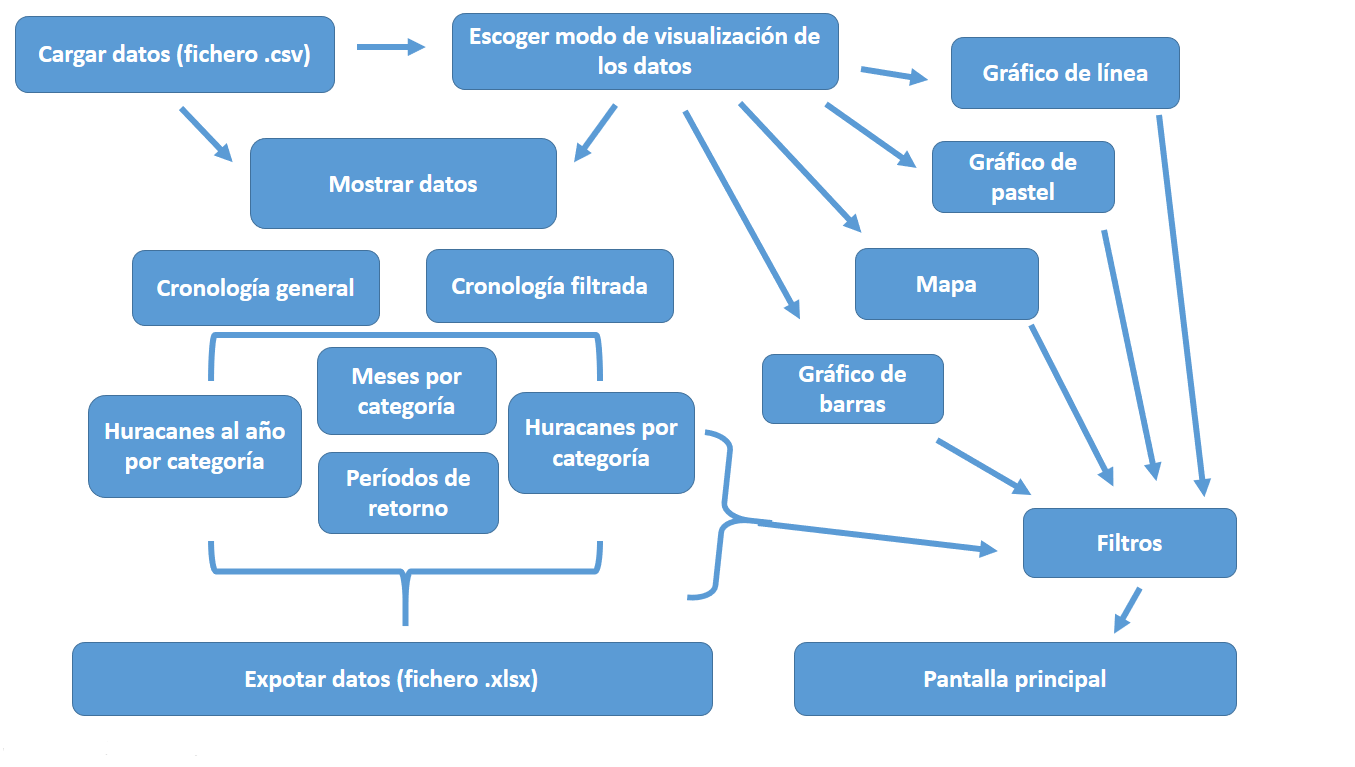
\includegraphics[scale=0.45]{esquema_metodologia}
\caption{Metodología seguida en el software TkHURSv1.1}
\label{fig:esquema_metodologia}
\end{figure}

\pagebreak

\section{Descripción del software}

\textbf{ TkHURSv1.1} es un software pensado para trabajar en él de forma intuitiva. Inclusive no cuenta con muchos comandos o botones para realizar la acción deseada con el objetivo de hacer su manejo lo más sencillo posible para el usuario. Es posible visualizar los datos en forma de tabla y gráfico lo que hace mucho más fácil las comparaciones o cualquier otro tipo de consulta que se quiera hacer con los datos proporcionados en el archivo ``.csv'' que se debió cargar previamente. 


\subsection{Pantalla principal}

Se brinda una breve descripción de las características del software que a nuestro entender son de gran importancia. La aplicación cuenta con una vista principal (Figura \ref{fig:Pantalla_principal_vacia}) compuesta por distintos componentes:
\\

\begin{figure}[H]
\centering
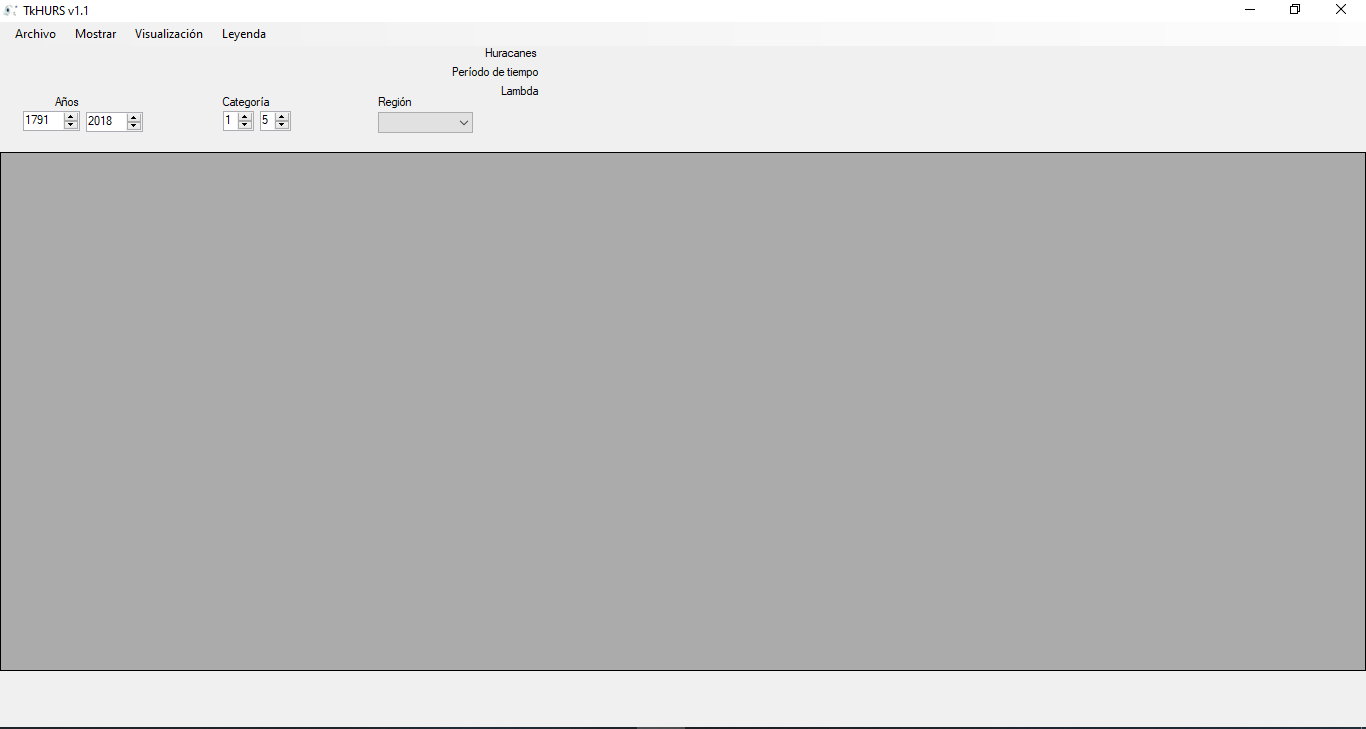
\includegraphics[scale=0.35]{Pantalla_principal_vacia}
\caption{Pantalla principal}
\label{fig:Pantalla_principal_vacia}
\end{figure}

\pagebreak

\begin{description}
\item[Archivo: ]{se usa para dos funciones: Cargar Cronología y Guardar.}

\item [Mostrar:] {se usa para seis funciones: Cronología General, Cronología Filtrada, Huracanes/Categoría, Huracanes Al Año/Categoría, Períodos de Retorno y Meses/Categoría.}

\item[Leyenda:] { esta pestaña se encarga de proporcionar la simbología usada en la aplicación.}

\item[Años:] permite elegir año de inicio y final para realizar distintos análisis sobre los datos.

\item[Categoría:]{ permite elegir una o varias categorías de los huracanes que se muestran.}

\item[Región:]{ permite elegir la provincia, la región o Cuba en general para realizar el análisis deseado.}

\item[Huracanes:]{ muestra la cantidad de huracanes.}

\item[Período de tiempo:]{ muestra la cantidad de años analizados.}

\item[Lambda:]{ muestra el valor estimado del parámetro poblacional lambda.}
\end{description}

\pagebreak

La imagen siguiente (Figura \ref{fig:Cronologia_general}) es otro de los estados de la aplicación: cuando se muestra la Cronología General surge otro elemento, el botón Guardar Cambios

\begin{figure}[H]
\centering
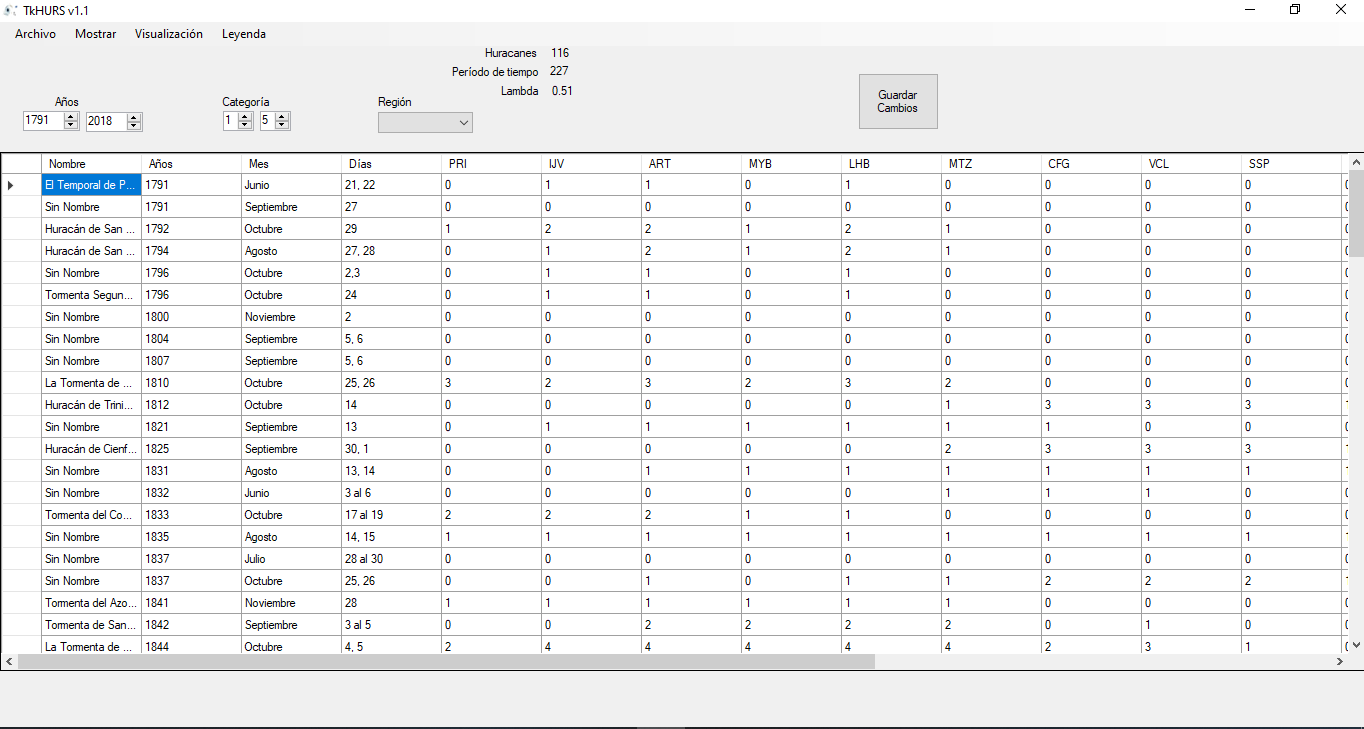
\includegraphics[scale=0.45]{Cronologia_general}
\caption{Pantalla principal con la cronología general cargada}
\label{fig:Cronologia_general}
\end{figure}


\begin{description}
\item[Guardar Cambios:]{ se usa para guardar cualquier cambio que se realice, creando un nuevo fichero que puede guardarse con el nombre deseado, sin afectar la cronología general.}
\end{description}

\pagebreak

\subsection{Entrada de los datos y descripción del fichero}

Parte principal del software es conocer los datos sobre los que se realizara el estudio. Para facilitarles a los usuarios la entrada de los mismos al programa se les brinda la opción de cargar un fichero ``.csv'' con la cronología, la cual se puede modificar y actualizar cada vez que sea necesario (Figura \ref{fig:Archivo_opciones}).


\begin{figure}[H]
\centering
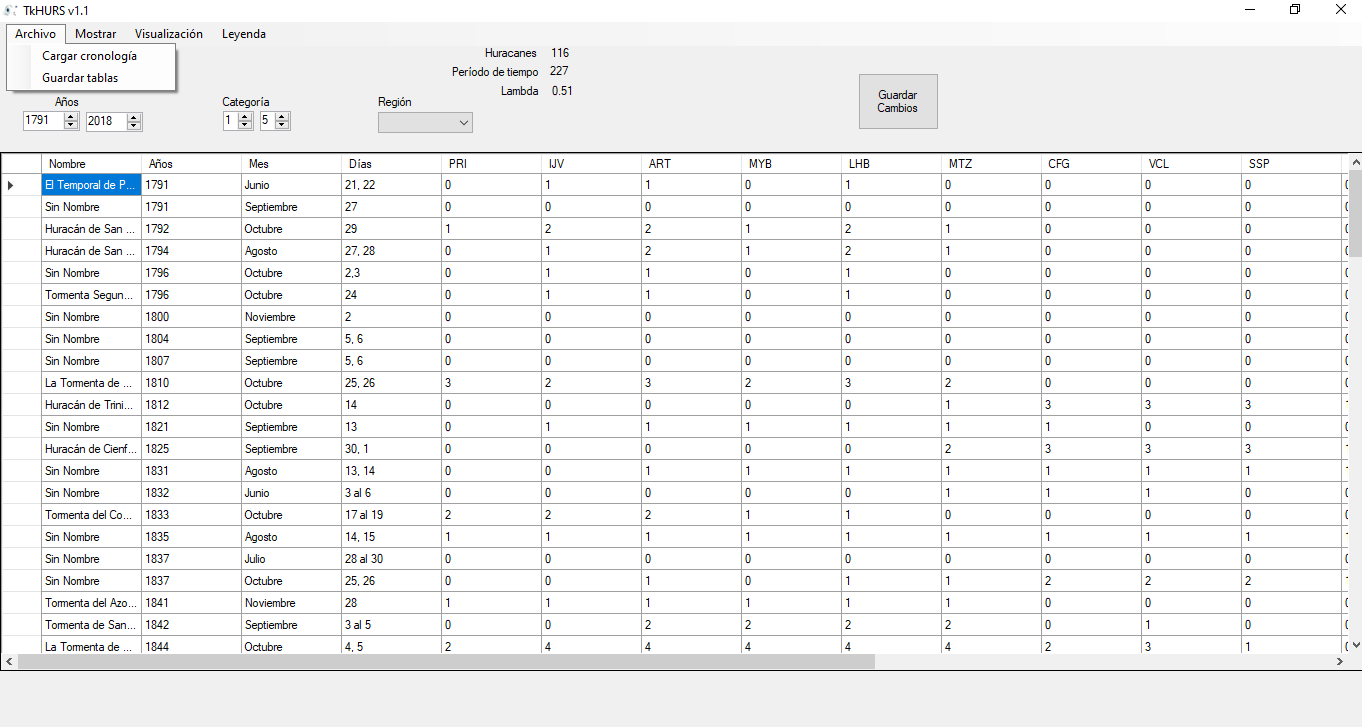
\includegraphics[scale=0.45]{Archivo_opciones}
\caption{Entrada de datos al sistema}
\label{fig:Archivo_opciones}
\end{figure}

\pagebreak

El fichero se describe de la siguiente manera: la primera columnas será el nombre del huracán, la segunda el año, la tercera el mes, la cuarta el o los días en que afectó al país y el resto de las columnas representarán con qué categoría afectó a cada una de las provincias. En caso de haber cargado los datos y querer seguir trabajando sobre ellos no es necesario volverla a cargar ya que la aplicación recuerda la última información cargada  (Figura \ref{fig:Fragmento_cronologia}).


\begin{figure}[H]
\centering
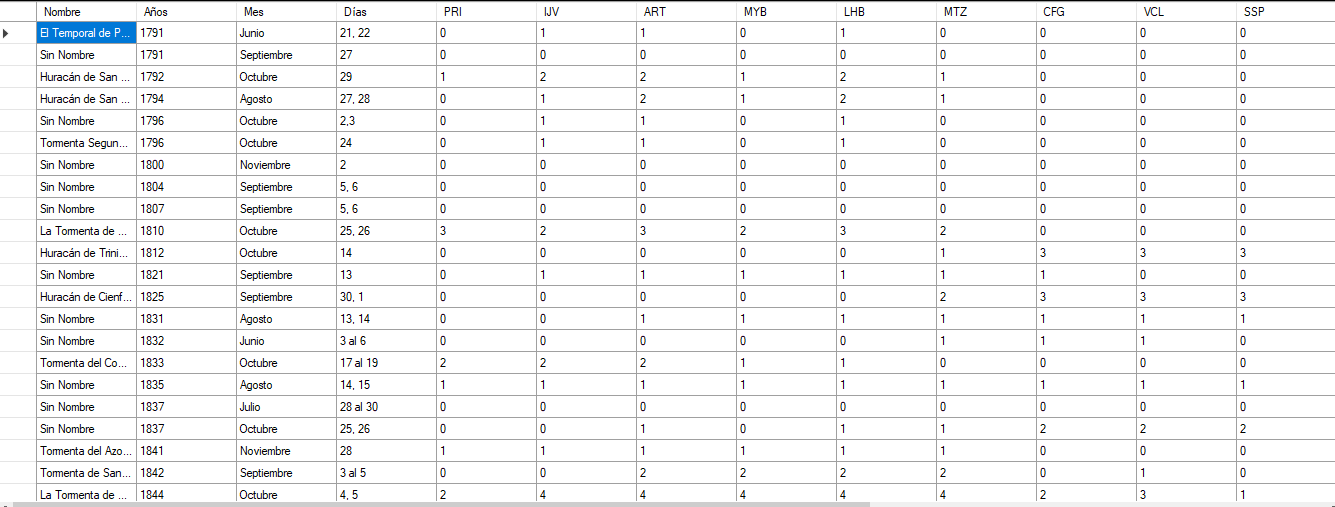
\includegraphics[scale=0.45]{Fragmento_cronologia}
\caption{Fragmento de la Cronología de huracanes de Cuba 1791-2018}
\label{fig:Fragmento_cronologia}
\end{figure}

\pagebreak

\subsection{Mostrar las distintas tablas y gráficos}

Con la opción ``Mostrar'' se pueden ver las distintas tablas acerca de los datos: Cronología General, Cronología Filtrada,Huracanes/Categoría, Huracanes Al Año/Categoría, Períodos de Retorno y Meses/Categoría (Figura \ref{fig:Mostrar_opciones}).\\

\begin{figure}[H]
\centering
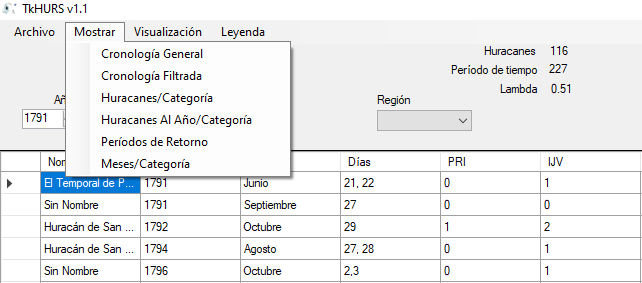
\includegraphics[scale=1]{Mostrar_opciones}
\caption{Se muestran las diferentes opciones de tabla}
\label{fig:Mostrar_opciones}
\end{figure}

Cada una de las vistas mencionadas con anterioridad van a ser explicadas con más detalle en breve para que se tenga una mejor idea del funcionamiento del software en cuestión \textbf{TkHURSv1.1}. Se espera que no haya dudas o al menos que se vean disminuidas después de esto.

\pagebreak

Cronología General: muestra la cronología cargada en su totalidad sin tener en cuenta filtros de ningún tipo (Figura \ref{fig:Cronologia_general1}). En esta vista es donde se pueden modificar y guardar los datos que se proveen en el archivo ``.csv''. Aquí es donde único se va a mostrar el botón ``Guardar Cambios'' que hace posible salvar las modificaciones realizadas.\\

\begin{figure}[H]
\centering
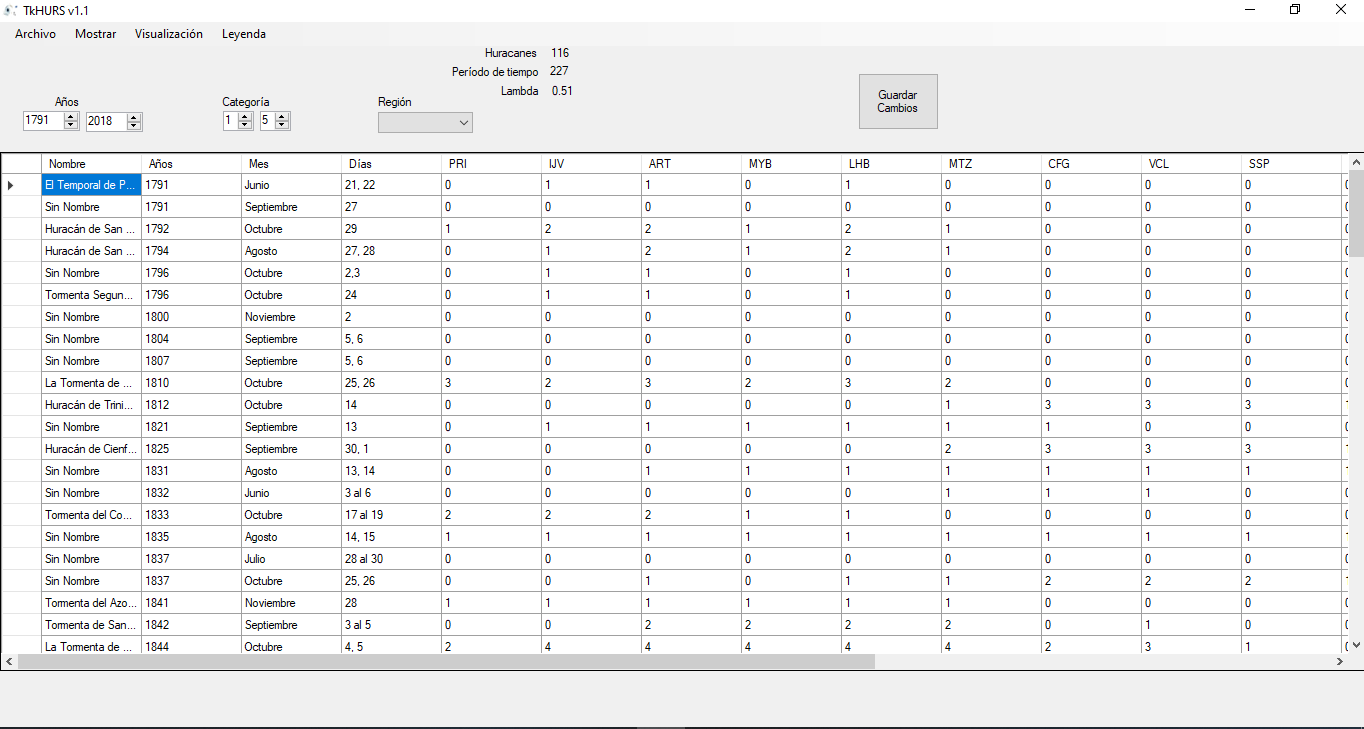
\includegraphics[scale=0.45]{Cronologia_general1}
\caption{Pantalla principal con la cronología general cargada}
\label{fig:Cronologia_general1}
\end{figure}

\pagebreak

Cronología Filtrada: muestra la cronología resultante de aplicar la selección de los datos del rango de años, de categoría y la región que se quiere investigar (Figura \ref{fig:Cronologia_filtrada}). Cabe destacar que a excepción de la opción ``Cronología general'', todas las opciones que siguen en lo adelante se ven afectadas por el filtro de la aplicación: el resto de las tablas, todos los gráficos y el mapa.\\


\begin{figure}[H]
\centering
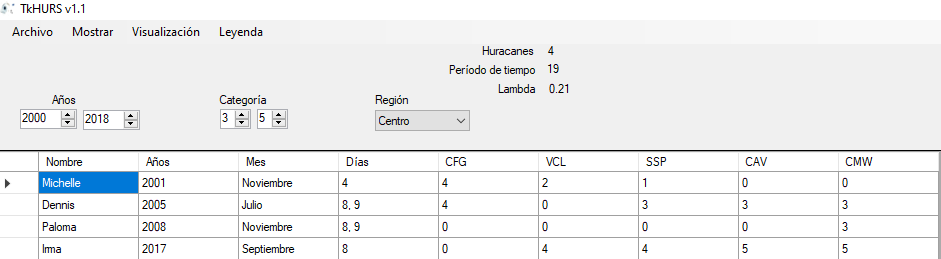
\includegraphics[scale=0.65]{Cronologia_filtrada}
\caption{Cronología filtrada}
\label{fig:Cronologia_filtrada}
\end{figure}

Huracanes/Categoría: muestra un conteo de los huracanes por categoría en la escala de Saffir-Simpson (Figura \ref{fig:Huracanes_categoria}).

\begin{figure}[H]
\centering
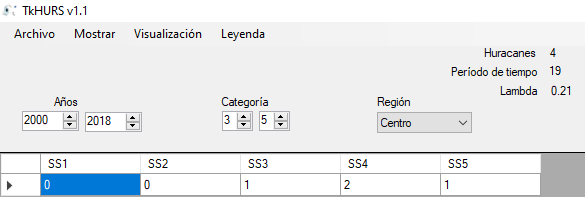
\includegraphics[scale=1]{Huracanes_categoria}
\caption{Huracanes por categorías}
\label{fig:Huracanes_categoria}
\end{figure}

\pagebreak


Huracanes al Año/Categoría: muestra un conteo de cuántas veces ha ocurrido cierta cantidad de huracanes al año de cada una de las categorías según la escala de Saffir-Simpson (Figura \ref{fig:Huracanes_ano_categoria}).

\begin{figure}[H]
\centering
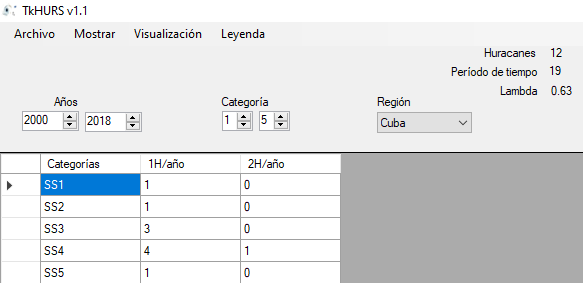
\includegraphics[scale=0.5]{Huracanes_ano_categoria}
\caption{Huracanes al año por categorías}
\label{fig:Huracanes_ano_categoria}
\end{figure}


Períodos de Retorno: esta es la función más importante de la aplicación porque aquí es donde se muestran los resultados calculados para el período de retorno de los huracanes para nuestro país; razón fundamental por la cual se decidió desarrollar esta aplicación de escritorio y por tanto parte vital en ella (Figura \ref{fig:Periodos_retorno}).

\begin{figure}[H]
\centering
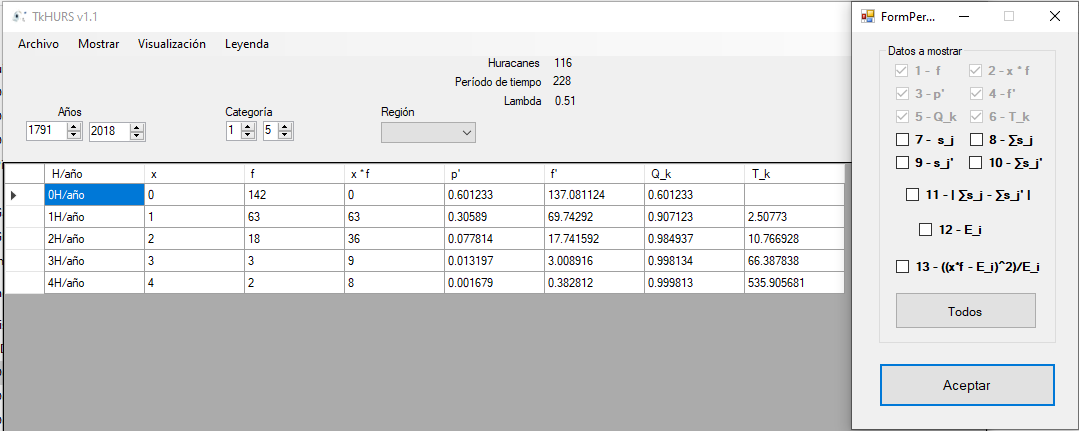
\includegraphics[scale=0.6]{Periodos_retorno}
\caption{Períodos de retorno}
\label{fig:Periodos_retorno}
\end{figure}

\pagebreak

Meses/Categoría: muestra un conteo de los huracanes por mes y categoría en la escala de Saffir-Simpson. Muestra en la última columna la cantidad de huracanes de los tres meses más activos (agosto, septiembre y octubre), sólo presenta ese valor; y la cantidad de huracanes intensos (categorías 3, 4 y 5 en la escala de Saffir-Simpson), valor observable en la última fila y solamente se ve ese resultado al igual que con los meses más activos (Figura \ref{fig:Meses_categoria}).

\begin{figure}[H]
\centering
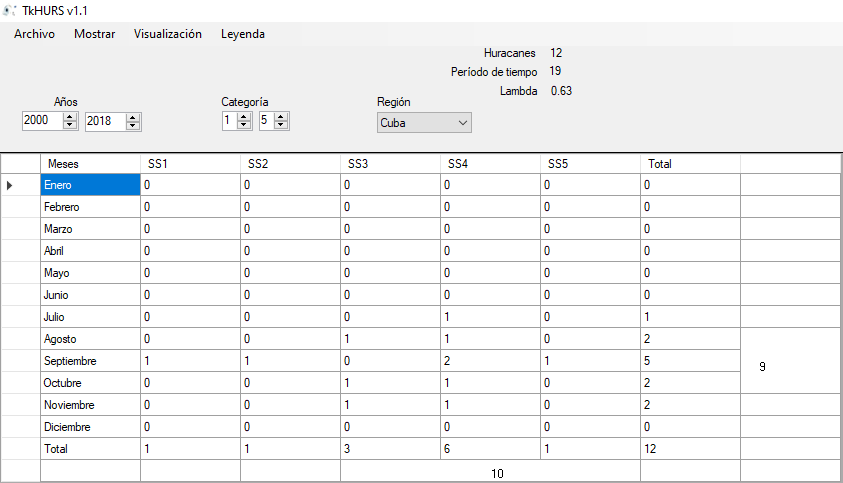
\includegraphics[scale=0.75]{Meses_categoria}
\caption{Meses por categoría}
\label{fig:Meses_categoria}
\end{figure}

\pagebreak

Visualización: muestra las opciones de vista que presenta el software; el “Modo Tabla” es para mostrar todos los datos de interés en dicho formato, “Modo Gráfico” tiene otras 3 opciones propias para elegir el tipo de gráfico en el que se quieran observar los resultados que se presentan en el archivo “.csv” (Gráficos de Barras, Pastel y Línea) y “Modo Mapa” (será implementada en la próxima versión) (Figura \ref{fig:Visualizacion}). %Fue pensado con el objetivo de permitirle al usuario analizar los datos desde distintos puntos de vista (Figura \ref{fig:Visualizacion}).\\

\begin{figure}[H]
\centering
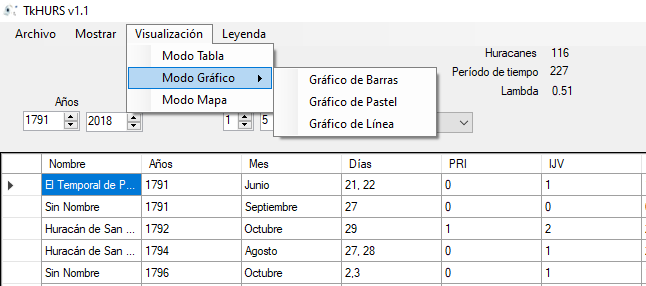
\includegraphics[scale=0.5]{Visualizacion}
\caption{Opciones de visualización}
\label{fig:Visualizacion}
\end{figure}


Gráfico de barras con la opción meses: el gráfico muestra el resultado del filtrado correspondiente luego de haber elegido los meses para el estudio (Figura \ref{fig:grafico_barras}). %Como se aprecia, es posible escoger de cúal en específico se quieren observar los resultados (Figura \ref{fig:grafico_barras}).

\begin{figure}[H]
\centering
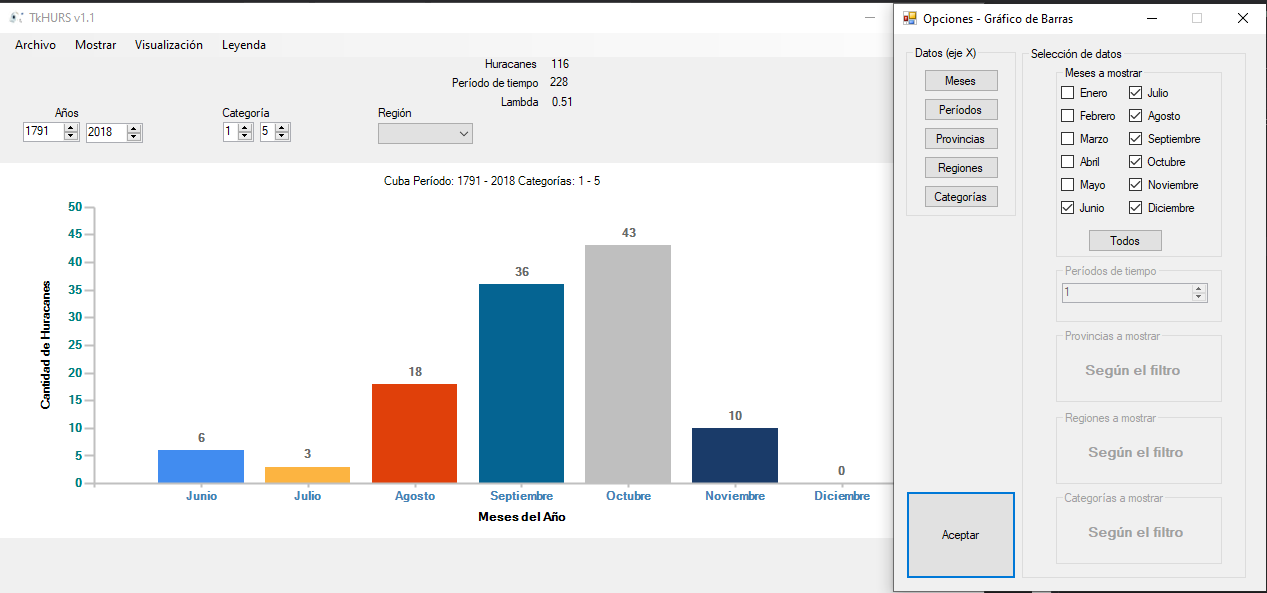
\includegraphics[scale=0.45]{grafico_barras}
\caption{Gráfico de barras (meses por cantidad de huracanes)}
\label{fig:grafico_barras}
\end{figure}

\pagebreak


Gráfico de barras con la opción período: el gráfico muestra el resultado del filtrado correspondiente luego de haber elegido el período de estudio. Como se aprecia, es posible escoger que rango de tiempo desea observar, haciendo sencilla la apreciación y el poder comparar distintos intervalos de tiempo en la historia cubana respecto a huracanes. En el ejemplo de la imagen se escogió un intervalo de 20 años (Figura \ref{fig:grafico_barras_periodo}).

\begin{figure}[H]
\centering
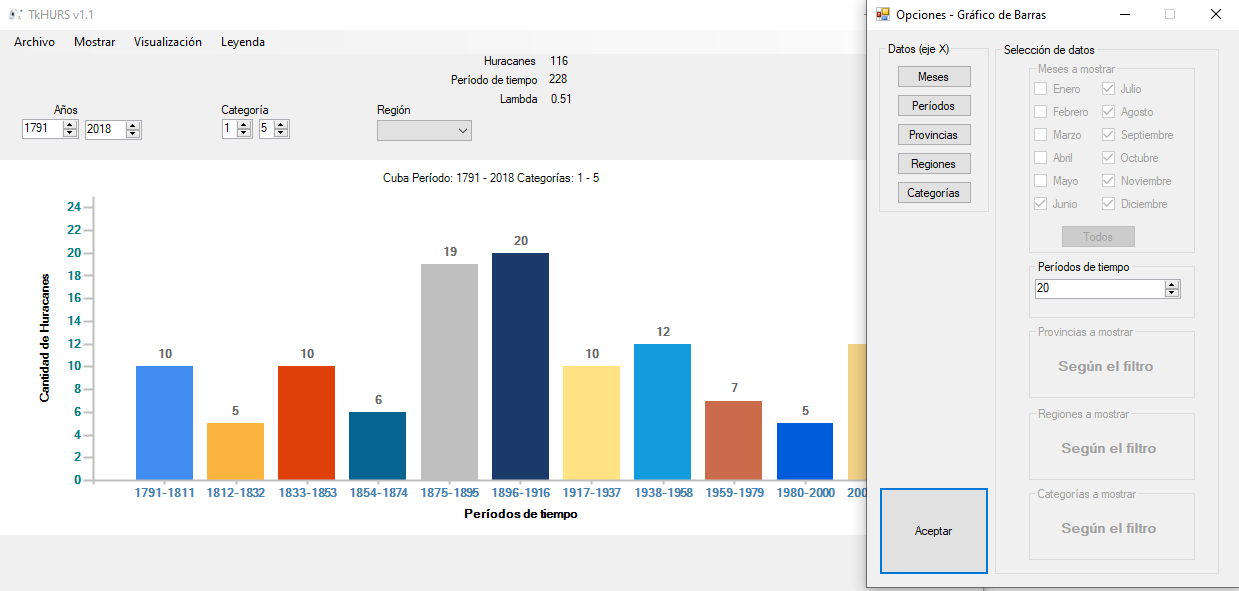
\includegraphics[scale=0.45]{grafico_barras_periodo}
\caption{Gráfico de barras (período de tiempo por cantidad de huracanes)}
\label{fig:grafico_barras_periodo}
\end{figure}

\pagebreak

Gráfico de barras: categorías por cantidad de huracanes, afectado por el filtro como la mayoría de las vistas. Muy útil permitiendo hacer la comparación entre las categorías de huracanes que afectan a Cuba. En la imagen se observa que, teniendo en cuenta la información dada en la cronología, no han llegado a La Isla muchos fenómenos tropicales del máximo valor en la escala de Saffir-Simpson (Figura \ref{fig:grafico_barras_categoria}).

\begin{figure}[H]
\centering
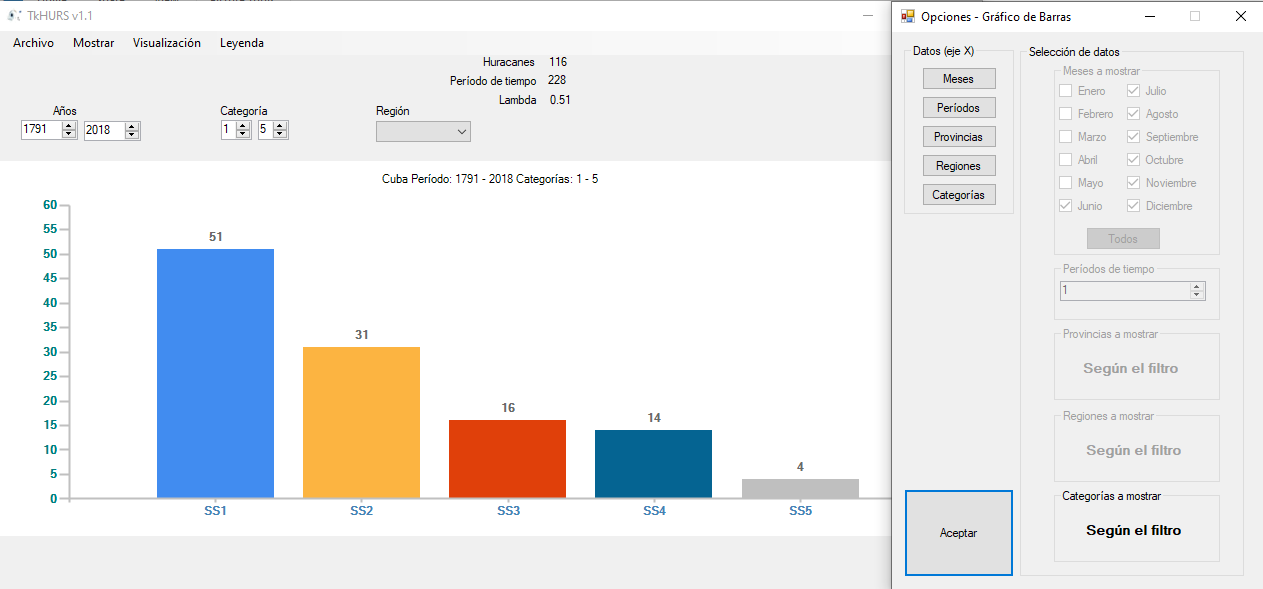
\includegraphics[scale=0.45]{grafico_barras_categoria}
\caption{Gráfico de barras (categorías por cantidad de huracanes)}
\label{fig:grafico_barras_categoria}
\end{figure}

\pagebreak

Gráfico de barras: se muestran las regiones por cantidad de huracanes e igual permite una rápida comparación. Es fácil apreciar cúal ha sido la región más afectada por los huracanes según los registros. Estas observaciones pueden ser de ayuda a la hora de establecer medidas preventivas con el objetivo de evitar pérdidas de vidas humanas y económicas, sabiendo las zonas más afectadas por estos fenómenos atmosféricos (Figura \ref{fig:grafico_barras_regiones}).

\begin{figure}[H]
\centering
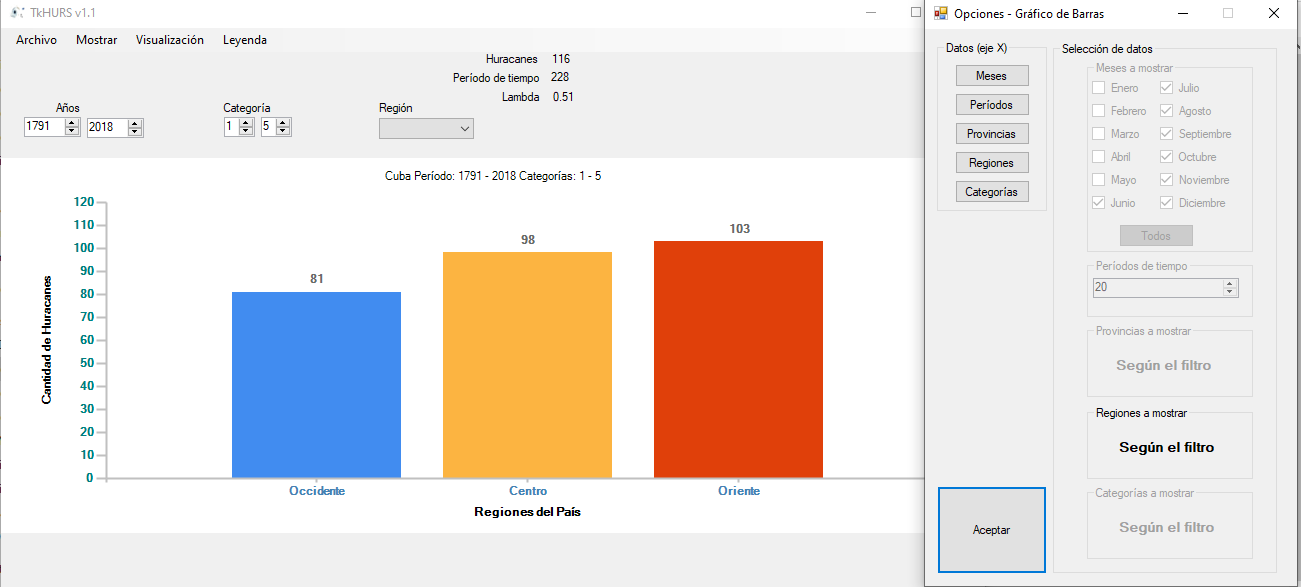
\includegraphics[scale=0.45]{grafico_barras_regiones}
\caption{Gráfico de barras (regiones por cantidad de huracanes)}
\label{fig:grafico_barras_regiones}
\end{figure}

\pagebreak

Gráfico de barras: provincias por cantidad de huracanes. Se aprecian las provincias (y municipio especial) y se puede observar que La Isla de la Juventud ha sido la más azotada por estos eventos meteorológicos a través del tiempo. Dato que no podríamos inferir sólo a partir del gráfico de regiones, por ejemplo (Figura \ref{fig:grafico_barras_provincias}).

\begin{figure}[H]
\centering
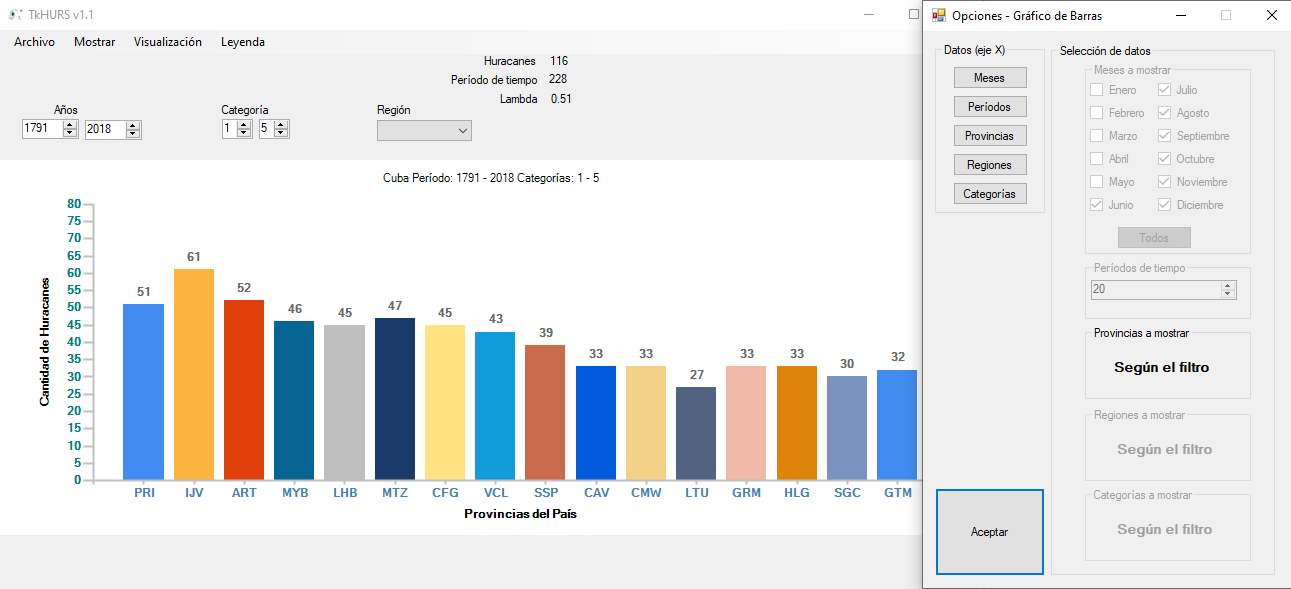
\includegraphics[scale=0.40]{grafico_barras_provincias}
\caption{Gráfico de barras (provincias por cantidad de huracanes)}
\label{fig:grafico_barras_provincias}
\end{figure}



Gráfico de línea: categorías por cantidad de huracanes (Figura \ref{fig:grafico_pastel_prcnt})

\begin{figure}[H]
\centering
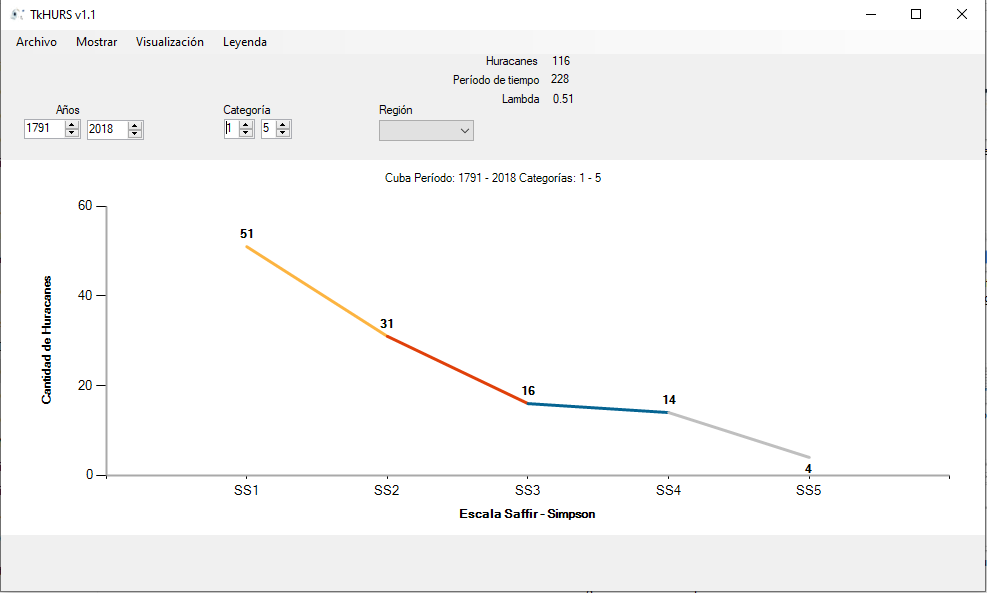
\includegraphics[scale=0.40]{grafico_lineas}
\caption{Gráfico de línea (categorías por cantidad de huracanes)}
\label{fig:grafico_lineas}
\end{figure}

\pagebreak

Gráfico de pastel: categorías por cantidad de huracanes (Figura \ref{fig:grafico_pastel_cant})

\begin{figure}[H]
\centering
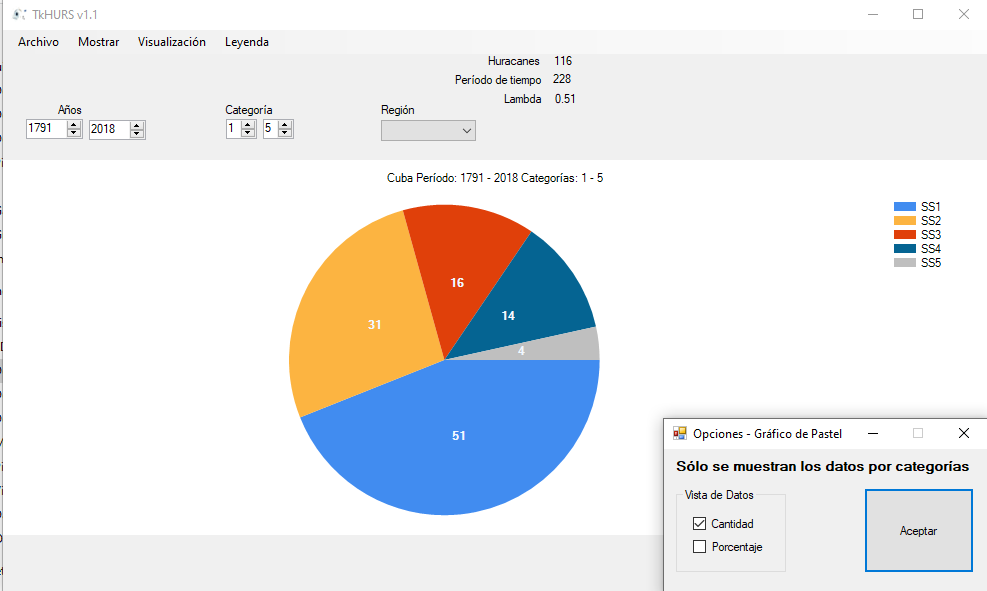
\includegraphics[scale=0.45]{grafico_pastel_cant}
\caption{Gráfico de pastel (categorías por cantidad de huracanes)}
\label{fig:grafico_pastel_cant}
\end{figure}

Gráfico de pastel: categorías por porcentaje de huracanes (Figura \ref{fig:grafico_pastel_prcnt})

\begin{figure}[H]
\centering
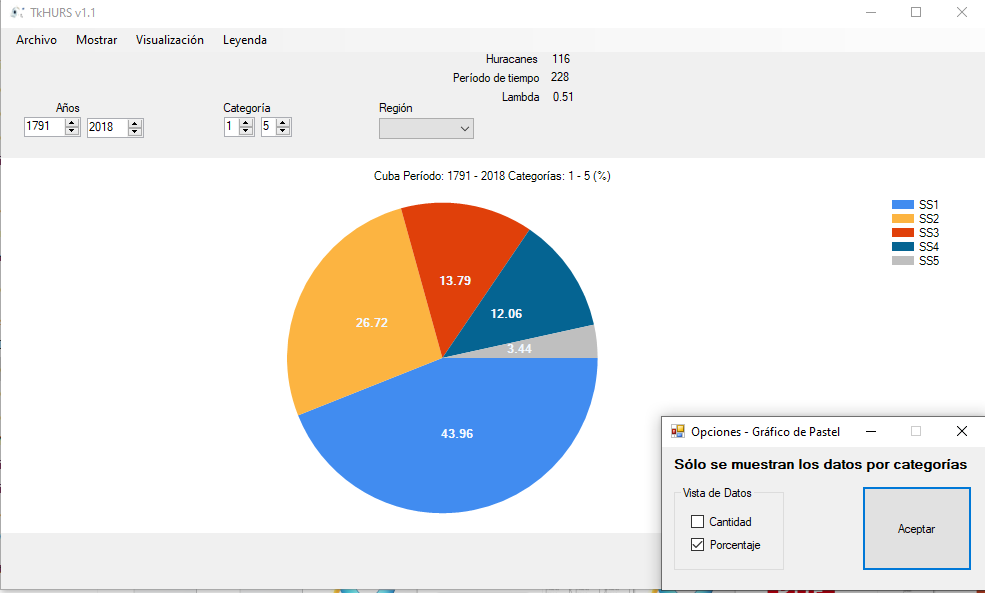
\includegraphics[scale=0.45]{grafico_pastel_prcnt}
\caption{Gráfico de pastel (categorías por porcentaje de huracanes)}
\label{fig:grafico_pastel_prcnt}
\end{figure}

\pagebreak


\subsection{Leyenda}

Esta pestaña se encarga de proporcionar la simbología usada en la aplicación. (Figura \ref{fig:Leyenda}).


\begin{figure}[H]
\centering
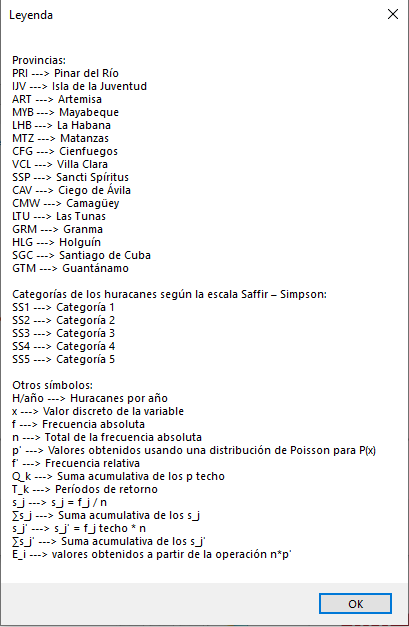
\includegraphics[scale=0.8]{Leyenda}
\caption{Leyenda de la simbología usada }
\label{fig:Leyenda}
\end{figure}

\pagebreak


\subsection{Exportar resultados}

Guardar: se exporta a un Excel toda la información obtenida o se salva una imagen del gráfico que se observe, depende de lo que esté en la pantalla principal. En la figura se observa el resultado de la primera opción (Figura \ref{fig:save}).


\begin{figure}[H]
\centering
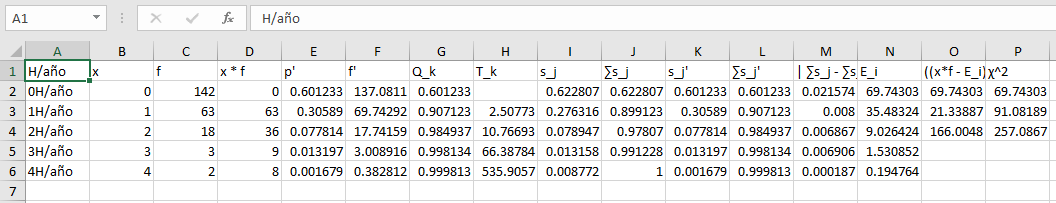
\includegraphics[scale=0.55]{save}
\caption{Datos guardados del análisis de períodos de retorno de huracanes }
\label{fig:save}
\end{figure}



























\chapter{Análisis y discusión de los resultados}
En este capítulo se exponen los resultados alcanzados en esta investigación y para ello se tomaron: un período de la cronología (1980 - 2018), algunas de las categorías del filtro (3 - 5) y una región del país (Centro), para procesar la información y observar los resultados que produce el software \textbf{TkHURSv1.1} para algunas de sus posibles salidas.\\

La primera imagen que se presenta es una parte de la cronología general (Figura \ref{fig:cronologia_general_parte}), el cambio respecto a las demás imágenes va a ser evidente porque la opción ``Cronología General'' es la única función en la aplicación de escritorio que no es afectada por los filtros

\begin{figure}[H]
\centering
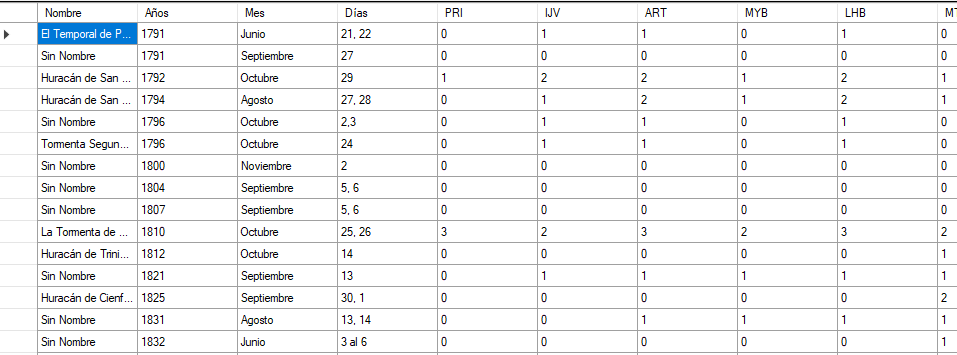
\includegraphics[scale=0.50]{cronologia_general_parte}
\caption{Fragmento de la Cronología de huracanes de Cuba (1791-2018)}
\label{fig:cronologia_general_parte}
\end{figure}

\pagebreak

La siguiente es la cronología filtrada a partir de las opciones escogidas que se mencionaron al principio (Figura \ref{fig:cronologia_filtrada19802018}). Por este resultado podemos conocer que la región Central de Cuba fue afectada por 4 huracanes en el rango de categorías elegido en la escala Saffir - Simpson durante el período de 1980 a 2018.


\begin{figure}[H]
\centering
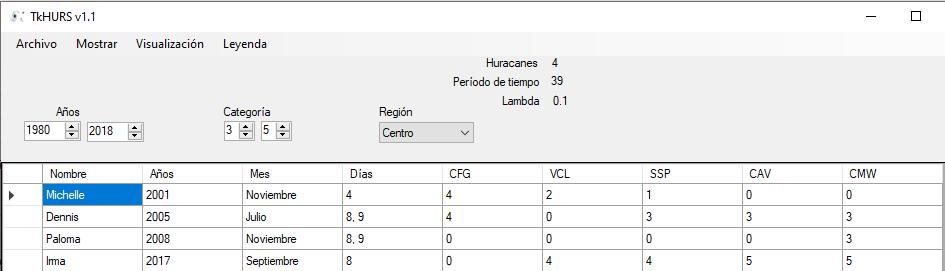
\includegraphics[scale=0.60]{cronologia_filtrada19802018}
\caption{Cronología filtrada, región Central de Cuba (1980-2018)}
\label{fig:cronologia_filtrada19802018}
\end{figure}

En la próxima imagen se muestran los huracanes por categoría (Figura \ref{fig:huracanes_categoria19802018}). Se aprecia que las categorías SS1 y SS2 tienen valor 0, resultado esperado dado que se dejaron fuera del rango de categorías seleccionado. 

\begin{figure}[H]
\centering
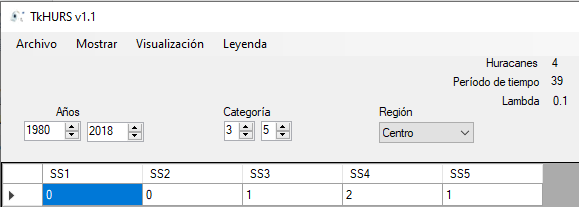
\includegraphics[scale=1]{huracanes_categoria19802018}
\caption{Huracanes por categorías intensas, región Central de Cuba (1980-2018)}
\label{fig:huracanes_categoria19802018}
\end{figure}

\pagebreak

Lo que se aprecia a continuación (Figura \ref{fig:periodos_retorno19802018}) es la tabla de períodos de retorno, donde se puede esperar que en la región Central pase un huracán intenso cada 10 años aproximadamente. %Las casillas que se exponen son las relacionadas con la prueba $\chi^{2}$ de Bondad de Ajuste, pero el usuario tiene la opción de ver los resultados relacionados con la prueba Kolmogorov-Smirnov que ya estaba disponible en el software desde la versión anterior.

\begin{figure}[H]
\centering
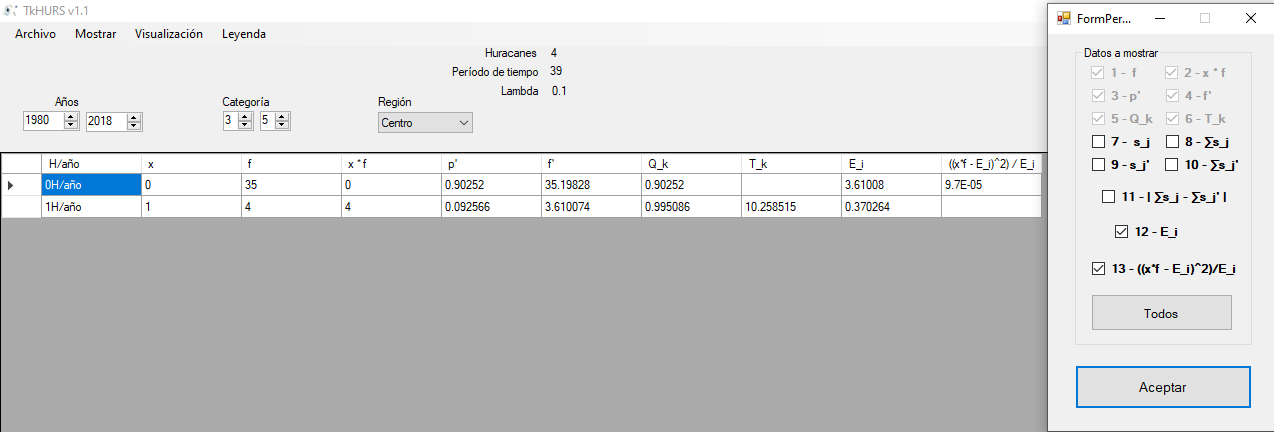
\includegraphics[scale=0.45]{periodos_retorno19802018}
\caption{Períodos de Retorno, región Central de Cuba (1980-2018)}
\label{fig:periodos_retorno19802018}
\end{figure}


El gráfico de barras muestra que en la región Central en la década del 2002-2012 fue el mas activo del período de estudio (Figura \ref{fig:barras_periodos19802018}). %Esta imagen (Figura \ref{fig:barras_periodos19802018}) muestra el gráfico de barras que se da como salida a partir de escoger dicho modo de visualización. Esto es de mucha ayuda: se observan, de manera clara, las diferencias entre los objetos de interés de estudio (intervalos de tiempo en este caso).

\begin{figure}[H]
\centering
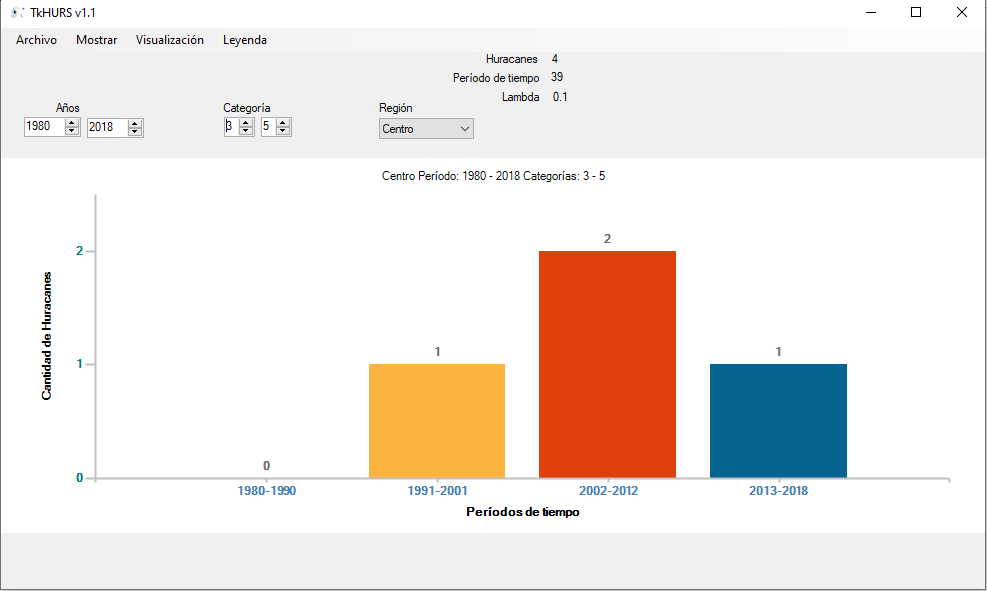
\includegraphics[scale=0.45]{barras_periodos19802018}
\caption{Gráfico de barras por décadas, región Central (1980-2018)}
\label{fig:barras_periodos19802018}
\end{figure}

\pagebreak

El gráfico de barras respecto a las provincias (Figura \ref{fig:barras_provincias19802018}) muestra como Sancti Spíritus y Camagüey han sido las más afectadas por los huracanes de categoria 3, 4 o 5 en la escala Saffir - Simpson en el período de 1980 a 2018.

\begin{figure}[H]
\centering
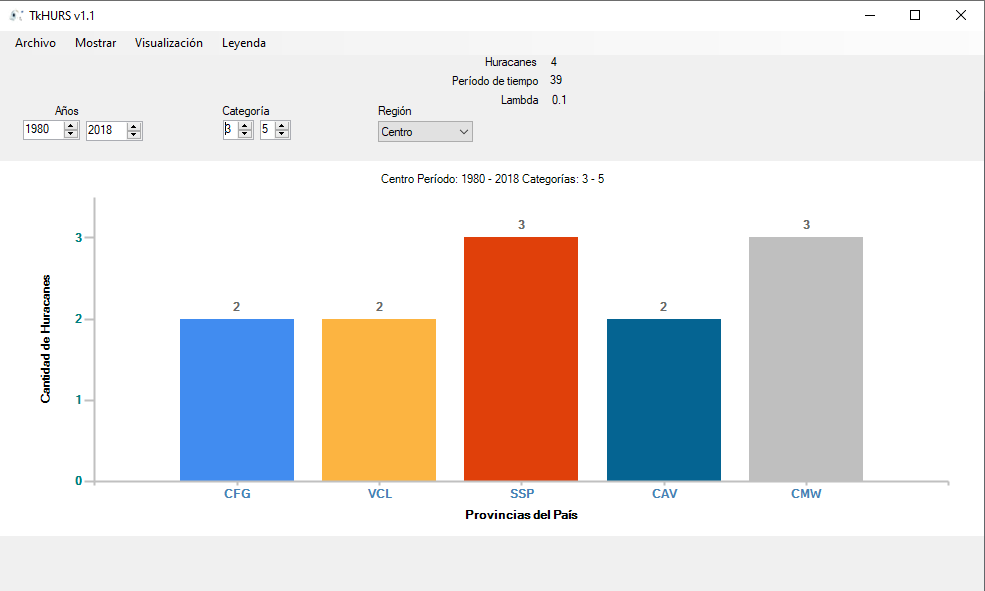
\includegraphics[scale=0.6]{barras_provincias19802018}
\caption{Gráfico de barras por provincias, región Central (1980-2018)}
\label{fig:barras_provincias19802018}
\end{figure}

\pagebreak

El gráfico de pastel en el software puede observarse en cantidad y porcentaje según se desee. Se muestra los resultados respecto a las distintas categorías: SS3, SS4 y  SS5. En este ejemplo se observa que la categoría que más ha afectado la región Central de Cuba es la cuarta (SS4) con un 50\% (Figura \ref{fig:pastel_porcentaje19802018}).%. El gráfico de pastel (Figura \ref{fig:pastel_porcentaje19802018}) solo muestra resultados respecto a las distintas categorías: SS1, SS2, SS3, SS4, SS5. Las opciones en este caso son: ``Cantidad'' y ``Porcentaje'', pero he escogido la segunda porque creo que aporta más visualmente. En este ejemplo se observa que la categoría que más ha afectado la región Central de Cuba es la cuarta (SS4) con un 50\%. 

\begin{figure}[H]
\centering
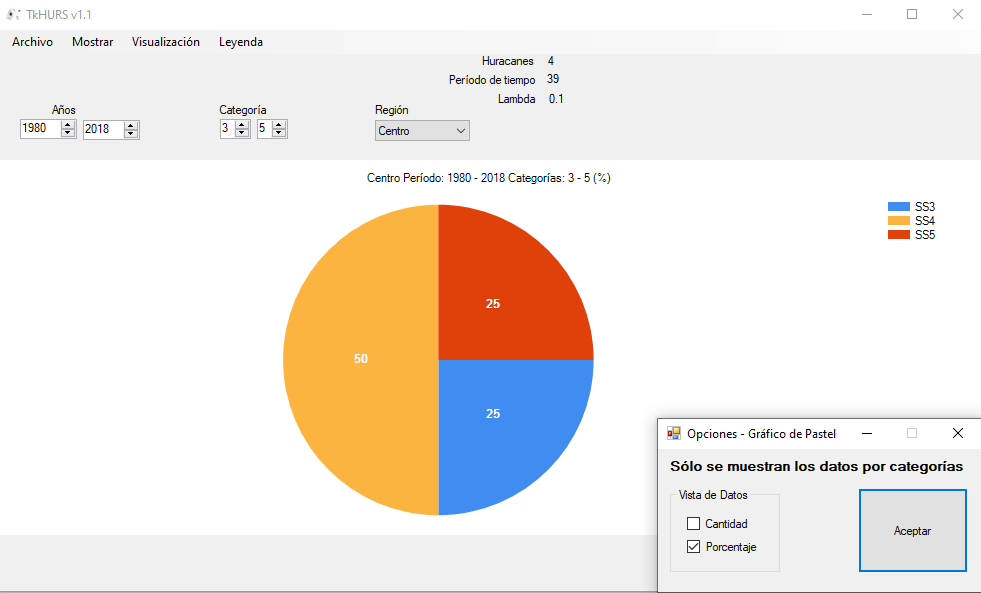
\includegraphics[scale=0.6]{pastel_porcentaje19802018}
\caption{Gráfico de pastel de las categorías en porciento, región Central (1980-2018)}
\label{fig:pastel_porcentaje19802018}
\end{figure}
%\chapter*{Conclusiones}


%\chapter*{Recomendaciones}
\label{chap:recom}

La investigación discutida en la tesis puede generalizarse
extendiendo la metodología propuesta a otros idiomas. Esto 
provoca cambios fundamentalmente en la etapa de preprocesamiento
donde se utilizan varios diccionarios y procesos que dependen del idioma 
utilizado~\footnote{diccionario de emoticones, diccionario de jerga, corrección 
ortográfica}. Para algunos de estos diccionarios se brinda una primera 
aproximación para idioma inglés, que no fue utilizada en este trabajo.
La metodología propuesta de manera general si es independiente del 
del idioma en el que estén los datos.

Para enriquecer los resultados propuestos pueden realizarse 
experimentos con nuevos algoritmos o variantes de los 
propuestos. En el trabajo se propone la utilización de algoritmos
estándares sin una parametrización exhaustiva de los mismos,
para poder realizar un análisis general de la propuesta. Por lo tanto 
pueden realizarse mejoras a los mismos.

El tamaño del corpus tiene una gran influencia sobre la precisión
de los resultados obtenidos. En consecuencia se propone continuar incrementando 
el corpus propuesto, utilizando la aplicación creada para la 
clasificación de mensajes. 

La tesis se concentra en la clasificación de mensajes sin tener en cuenta 
información semántica de los mismos. Una propuesta a largo 
plazo puede incluir clasificadores que utilicen información adicional
como los emoticones, relaciones de sinonimia, aparición de signos de puntuación 
especiales y conocimiento sobre los términos~\footnote{Puede utilizarse información
sobre la polaridad del término o el papel gramatical que ocupa~(adjetivo, sustantivo, verbo)}.

El proyecto resultante de este trabajo está concebido
como parte de un proyecto general que se está desarrollando en el
grupo de investigación. Es por tanto necesario integrar
de forma efectiva la metodología propuesta en el
entorno de análisis de información sobre
\emph{Twitter} que se encuentra en desarrollo.



%\include{MainMatter/Corpus}
%\chapter{Normalización de los Datos}
\label{chap:prep}

Un \emph{Tweet} es un mensaje de 140 caracteres donde es común encontrar gran uso de abreviaturas y jerga
de la web, por lo general para expresar opiniones se utiliza gran diversidad de emoticones y se deforma el
lenguaje ya que la ortografía y la gramática del idioma no son muy relevantes en estos mensajes. Es muy
usual que porten etiquetas y marcas propias de \emph{Twitter} como las de usuario, tópicos o \emph{reTweet}~(utilizado
para indicar que algún usuario replicó el mensaje) y que hagan referencia a diferentes sitios de la web.

\begin{verbatim}
bloggerscuba >Ya vieron el artículo de Global Voices? http://bit.ly/7uPumv

yudivian jajaja :D

RT yudivian: Vas a estar pa record roger213tm dos #nutella 
in one week &lt;- Por lo menos tremendo average :P

RT MaiteLpez: caroboris NUnca estare en el grupo de industriale 
sen Facebook ni en ningun lugar #VillaClara campeon &lt;- #EPD

RT: oxigeno: roger213tm por las #torticas!! &lt;- SSSSSufre... ajaja

nos perdimos de aki jijiji

&lt;(o-o)&gt;
\end{verbatim}

En la web los mensajes no están sujetos a estrictas reglas sintácticas del lenguaje \cite{Merlo2010} lo que dificulta la
aplicación de algoritmos de minería de opinión sobre ellos. Por tanto se propone un proceso de conversión
de los \emph{Tweets} a lenguaje natural. La primera diferencia de un \emph{Tweet} con un texto en lenguaje natural es
el uso indiscriminado de abreviaturas y jerga utilizada en la web debido a la restricción en la longitud de
140 caracteres.La jerga también llamada \emph{netspeak}~(uso informal de palabras y expresiones que no están
consideradas en el idioma o dialecto del hablante) ofrece como resultado más de una abreviatura para
una única palabra lo que en el entrenamiento provoca que el peso de la palabra quede repartido entre las
variaciones de la misma o en la clasificación una de las variaciones obtenga un peso mínimo aunque la
palabra esté entre los términos determinantes a la hora de clasificar. Por tanto es evidente la necesidad de
traducir la jerga a un lenguaje más convencional, para esto se propone el uso de diccionarios en diferentes
idiomas~(español e inglés) de la forma: jerga--idioma que se consultará para la conversión.

También es frecuente la utilización de emoticones o \emph{smileys} empleados para darle expresividad al
mensaje dado que internet es un medio frío y a menudo se desean expresar opiniones positivas o negativas.
A los emoticones se le da usos más complejos de detectar como es la ironía, de ahí que sean muy
importantes al realizar un análisis de sentimientos. Se dispone de un diccionario con 144 emoticones y
las frases que definen su semántica lo más breve posible.
Como parte del preprocesamiento se hace tratamiento para evitar las diferencias entre mayúsculas y
minúsculas que pueden suponer diferencias para el ordenador cuando realmente se hace referencia a la
misma palabra~(Ejemplo: Hola, hola, hOlA, HOLA). Este paso consiste simplemente en convertir todo
a minúsculas.

Una deformación común en internet es la modificación de la sintaxis de las palabras repitiendo
caracteres dentro de la misma con el objetivo de enfatizarla~(Ejemplo: "hooooooola"). Generalmente
la mayor o menor presencia de este efecto está muy ligado al tipo de contenido con que se trabaja y
dentro de este al estilo propio del autor. En las páginas de noticias escritas por periodistas normalmente
hay un mayor control de la ortografía mientras que las páginas de reseñas o en los blogs este fenómeno
es mucho más frecuente y en \emph{Twitter} su presencia se acentúa todavía más ya que en este lenguaje no
es relevante la ortografía. Para un análisis posterior del texto es necesario suprimir las letras repetidas,
pero existen palabras correctas con más de un carácter igual consecutivo~(Ejemplo: \emph{good}, acción). Por
lo tanto se propone suprimir los caracteres repetidos hasta dos ocurrencias. Existe otro problema y es
que no todas las palabras con 2 caracteres repetidos son transformadas y pueden haber sido escritas
incorrectamente por lo que llegado a este punto se utiliza un corrector ortográfico que determine las
palabras correctas. Si el corrector da más de una forma correcta para la misma palabra esta se deja como
está en el texto al igual que si no se encuentra ninguna forma correcta y se continua con el proceso de
análisis.

En \emph{Twitter} es relativamente común la utilización de referencias a otros sitios de la web con frecuencia
blogs, noticias o reseñas. La dirección de estos sitios, generalmente acortada usando un servicio específico
para ese fin, aparece en el propio mensaje. El problema surge cuando en la URL se encuentran palabras
que pueden influir sobre el clasificador de forma no deseada. Por esto es necesario eliminarlas ya que
forman parte del texto del mensaje
En un \emph{Tweet} se hace referencia no solo a sitios de internet, también pueden hacerse referencias a
otros usuarios de \emph{Twitter} a un tópico en especial o a otros \emph{Tweets} mediante el uso de marcas o etiquetas
propias de \emph{Twitter} que aparecen en el texto y pueden influir de la misma manera que las URL sobre los
clasificadores por lo tanto también son eliminadas.
Al finalizar este preprocesamiento se considera que el \emph{Tweet} se encuentra en lenguaje natural y se
respetan los signos de puntuación que serán utilizados en análisis posteriores.

%--------------------------------
Como se describe anteriormente el determinar el idioma del \emph{Tweet} permite cargar los diccionarios de
archivos de texto, según el idioma determinado. Aunque en una primera etapa solo se considerarán
mensajes en Español y posteriormente en Inglés. También se carga por defecto el diccionario de emoticones
que no depende del idioma del texto. Los diccionarios están almacenados en archivos de texto~(de la forma
jerga/emoticon : significado):

\begin{verbatim}

CU2MORO : ”See you tomorrow”

Googlear : Buscar en Google

:-] : positivo

’] :’ : negativo
\end{verbatim}

El procesamiento sobre el \emph{Tweet} es eliminar las etiquetas de \emph{Twitter} y las URLs mediante un autómata
finito determinista que elimina todos los caracteres detrás de un $\sharp$ o que se reconozca como
la dirección de un sitio. También se elimina la etiqueta ”RT” si se encuentra en cualquiera de sus
formas~(rt, Rt, rT) y si está rodeada de espacios ya que de lo contrario se pueden eliminar partes de
palabras correctas.
Para identificar los emoticones se propone el uso de expresiones regulares y el diccionario de emoticones
para crearlas. Estos son eliminados del texto para que no se confundan con la jerga o signos de
puntuación y evitar que cambien de sentido debido a otras transformaciones.
Para analizar el texto es necesario encontrar una unidad básica~(en nuestro caso utilizamos las palabras. 
Se entenderá por palabra inicialmente el resultado de dividir el \emph{Tweet} por espacios. Luego cada
palabra es verificada contra el diccionario de jerga después de convertirla a minúsculas y si no se considera
jerga se divide la palabra en los grupos continuos de puntuación y de caracteres alfabéticos donde
los últimos continúan siendo procesados como palabras nuevas.
Las nuevas palabras se vuelven a comparar con jerga y se les suprimen los caracteres repetidos hasta
dos ocurrencias para luego verificar la palabra correcta mediante los algoritmos de corrección ortográfica.

\section{Stemming}
Para el \emph{stemming} se propone una variante del algoritmo de Porter para Español de la 
librería nltk. Al algoritmo original se le hicieron varios cambios:
\begin{itemize}
 \item Considerar los sufijos: ito ita azo aza itos itas azos azas
 de los diminutivos y aumentativos.
 \item Se agrega la regla de que estos sufijos solo se podrán eliminar si lo que queda de la palabra es
 mayor o igual a tres caracteres.
 \item Se agrega la regla de que estos sufijos solo se podrán eliminar si al agregar la 
 última letra del sufijo al resto de la palabra, esta tiene sentido~(aparece en los diccionarios).
\end{itemize}

Ejemplo:

perr\emph{ito} 
perro (aparece en el diccionario)
--------------
perr

suscr\emph{ito}
suscro (no aparece en el diccionario)
------------
suscrit

\section{Stop Words}

Las \emph{stop words} son palabras que serán eliminadas una vez que sean encontradas en el texto.
Para esto se trabajo en un listado de palabras propuestas en diferentes sitios de internet 
como las \emph{stop words} más utilizadas, pero varias de estas palabras pueden aportar 
semántica a la opinión que se da en el mensaje. Por lo tanto se propone no incluir:

\begin{center}
\begin{tabular}{c c c}
  no & muy & ni \\
  si & contra & algunos \\
  pero & tanto & algunas \\
  más & mucho & poco \\ 
  como & nada & algo \\ 
  tanto & muchos & entonces \\
  cierto & bajo & verdad \\
  ciertos & arriba & verdadero \\
  ciertas & encima & verdadera \\
  cierta & valor & modo \\
  bien & mientras & \\
\end{tabular} 
\end{center}


%\chapter{Clasificación}
\label{chap:clas}

	La clasificación de los mensajes se divide en dos etapas:
	
	\begin{itemize}
	\item Determinar si el mensaje es objetivo o subjetivo.
	\item Clasificar los mensajes subjetivos en positivos o negativos.
	\end{itemize}
	
	Se propone la experimentación con los mismos clasificadores en las dos
	etapas, ya que ambas enfrentan el mismo problema teórico.

	El aprendizaje supervisado parece una alternativa natural para enfrentar este
	problema, ya que se desea asignar a cada mensaje una clasificación única.
	El conjunto de entrenamiento se construye a partir de la clasificación
	manual por parte de especialistas~(en este caso los autores) de una lista
	de \emph{tweets} extraídos del sitio de \emph{Twitter} empleando herramientas
	desarrolladas en la facultad para este propósito. Es necesario notar que 
	incluso la tarea de clasificación manual es difícil, debido a la ambigüedad
	inherente a estos mensajes. Por este motivo se ha escogido~(intentado confeccionar
	un conjunto de entrenamiento seleccionando) los mensajes que para un humano
	tienen una orientación bien definida, obviando los mensajes donde los clasificadores
	humanos estuvieron en desacuerdo.
	
	Los clasificadores empleados reciben un conjunto de entrenamiento en 
	la etapa de aprendizaje, que en este caso es obtenido a partir de un archivo de
	texto con una entrada por línea de la forma
	\verb|MENSAJE ====> CLASE|, donde la clase asignada es \verb|OBJETIVO|,
	\verb|NEGATIVO| o \verb|POSITIVO|.
	
	Existen varios algoritmos de clasificación, teniendo en cuenta el problema que se desea 
	resolver se eligieron para probar aquellos que son más recomendados en la literatura:
	\begin{itemize}
	    \item Naive Bayes.
	    \item Máquinas de soporte vectorial~(SVM).
	    \item Redes Neuronales.
	    \item K vecinos más cercanos.
	    \item Árboles de decisión.
	    \item Redes Bayesianas.
	    \item Máxima entropía.
	\end{itemize}
  
	La mayoría de los clasificadores utilizados forman parte de la herramienta \emph{sklearn}.
	La que cuenta con gran variedad de algoritmos de aprendizaje. Además contiene operaciones y estructuras
	de datos diseñadas para trabajar con vectores esparcidos y realizar validaciones sobre los resultados
	obtenidos. 
	

  
%\chapter{Estado del Arte}
\label{chap:basis}

\section{Gestión de redes}
\label{sec:network_management}
 Las redes de computadoras han evolucionado con el paso del tiempo ante la
necesidad de satisfacer las demandas de los diferentes servicios de
telecomunicaciones. Es por esto que cada día se requiere un mayor ancho de banda
y una mejor calidad del servicio para las nuevas aplicaciones que se han venido
desarrollando hasta la actualidad. La tecnología de las redes ha incrementado su
complejidad generándose la necesidad de contar con una mejor administración de
sus recursos, lo cual ha favorecido la evolución conjunta de la gestión de
redes. 

Según la perspectiva del usuario, la gestión de redes tiene diferentes
significados. Para algunos podría consistir simplemente en tener a un
especialista monitorizando los servicios o protocolos desactualizados con el
objetivo de mantenerlos actualizados. Para otros, involucra una base de datos
distribuida y estaciones finales que generan en tiempo real gráficos de los
cambios de la topología de la red y el tráfico. En resumen, se puede decir que
es un mecanismo que emplea una variedad de herramientas, aplicaciones y
dispositivos con el objetivo de asistir a sus administradores en la
monitorización y el mantenimiento de la red.

Una definición puede ser la siguiente\cite{Saydam1996}:
\begin{quotation}
 \emph{``La gestión de redes incluye el despliegue, integración y coordinación
del hardware, software y los elementos humanos para monitorizar, probar,
sondear, configurar, analizar, evaluar y controlar los recursos de la red para
conseguir los requerimientos de tiempo real, desempeño operacional y calidad de
servicio a un precio razonable.''}
\end{quotation}

Adicionalmente, al reducir lo tiempos de inactividad y minimizar los efectos de
las interrupciones, la gestión mantiene en buen estado la red, aumentando el
nivel de satisfacción de los usuarios que en definitiva son quienes trabajan en
las computadoras para utilizar los servicios ofrecidos.

En respuesta a la expansión de las redes y al rápido crecimiento de Internet,
diversas organizaciones internacionales han desarrollado iniciativas para la
gestión automatizada de los recursos de la red que luego se han convertido en
normas\cite{Exposito2003}. Cada una de estas normas describe una arquitectura
con ciertas características, pero en general, todas incluyen estaciones finales
(los elementos a ser gestionados, como computadoras y dispositivos de red) con
un \textit{software} incorporado que les permite alertar a las entidades de
gestión o nodos gestores de la existencia de algún problema. Por su parte, estas
pueden realizar encuestas a las estaciones finales y así analizar ciertos
valores previamente almacenados en estas. Esto se conoce como el paradigma
gestor-agente. %TODO: Poner ref a este paradigma

Las encuestas realizadas por las entidades de gestión pueden ser automáticas o
iniciadas por el usuario y los agentes en los dispositivos gestionados responden
a todas. Los agentes son módulos de \textit{software} que primero compilan
información acerca de los dispositivos gestionados en los cuales ellos residen.
Luego, almacenan esta información en base de datos y finalmente la proveen de
forma proactiva o reactiva a los nodos gestores a través de protocolos de
gestión. Existe un variado número de protocolos que tienen como objetivo el
soporte de la red y la gestión de los dispositivos que a ella pertenecen. Estos
protocolos incluyen a SNMP\cite{Hardaker2011} y a RMON\cite{Fenner2005}.

Usualmente en su funcionamiento una plataforma para la gestión de la red recibe
y procesa eventos de los elementos de red que la conforman. Aunque los
servidores y los demás recursos que la componen también pueden enviar eventos a
dicha plataforma. Generalmente estas cuentan con las siguientes funcionalidades:
\begin{itemize}
 \item Descubrimiento o reconocimiento de la red.
 \item Reconocimiento de los elementos de la red.
 \item Manejador o gestor de eventos.
 \item Desarrollo de un recolector de datos y un graficador de la red.
 \item Navegador de la gestión de datos.
\end{itemize}

En consecuencia las plataformas para la gestión de la red pueden ser vistas como
la aplicación principal para las operaciones en la detección de fallas en
la infraestructura de las redes. Algunas de las aplicaciones existentes en este ámbito tan
sólo presentan a los administradores un gráfico de la topología de la red, donde
se puede apreciar el estado de cada una de sus componentes. 

Las tareas asociadas al proceso de gestión de red fueron formalmente
especificadas por la organización conocida como Interconexión de Sistemas
Abiertos (OSI)\footnote{Por sus siglas en inglés, \textit{Open Systems
Interconnection}} de la Organización Internacional para la Estandarización 
(ISO)\footnote{Por sus siglas en inglés: \textit{International Organization for
Standardization}. \\ \url{http://www.iso.org/}}, con lo cual se puede esperar
interoperabilidad entre los sistemas de gestión que cumplan con dicha
especificación. La ISO definió cinco áreas funcionales o disciplinas dentro de
la gestión de red. Estas son:

\textbf{Gestión de la configuración} Sus tareas fundamentales son: la
recolección de datos sobre el estado de la red, su utilización para actuar sobre
la configuración de los recursos gestionados y el almacenamiento de los datos
sobre la configuración de la red (base de datos utilizada por el resto de las
áreas funcionales). Puede ser considerada como el área funcional más importante
pues las tareas asociadas a las otras cuatro áreas se basan, en mayor o menor
medida, en datos recogidos y mantenidos por este tipo de gestión. %TODO: Poner ref a 10 y 3 de idis

\textbf{Gestión de prestación o comportamiento} Su objetivo principal es el
mantenimiento del nivel de servicio que la red ofrece para lograr su
operabilidad en todo momento. Tiene mucho que ver con el tráfico existente en la
red. Permite además conocer de qué forma se emplean los recursos, con lo cual se
tienen elementos de juicio para la futura evolución de la red y saber qué tipo
de inversiones son las más adecuadas. %TODO: Poner ref a 10 y 12 de idis

\textbf{Gestión de fallos} Su objetivo principal es la localización y solución
de los problemas que presente la red, ofreciendo un soporte preventivo y
correctivo a su funcionamiento. Permite, en muchas ocasiones, detectar y
subsanar los problemas antes de que se percaten los usuarios. %TODO: Poner ref a 10 y 5 de idis.

\textbf{Gestión de seguridad} Es la responsable de controlar el acceso a los
recursos de la red, de acuerdo a ciertas directivas, para que las mismas no sean
boicoteadas de ninguna manera. La información que está en la red solo es
accedida por el personal autorizado y en el momento deseado. %TODO: Poner ref a 10 y 17 de idis.

\textbf{Gestión de la contabilidad} Conocida también como gestión de los
recursos, se encarga de contabilizar el uso de estos para valorar el costo del
consumo. Permite cobrar los servicio ofrecidos y amortizar con ello las
inversiones realizadas y los costos de los ofrecidos por terceros. Ayuda además
a tener elementos de decisión para una asignación de recursos de una manera más
eficiente. %TODO: Poner ref a 10 y 1 de idis.

Para los fines del presente trabajo, el cual se propone diseñar e implementar un
sistema distribuido para la detección de anomalías, se profundizará en los
sistemas de gestión de fallos, tarea en la que queda enmarcado el mismo. Como se
aprecia anteriormente los objetivos principales en la gestión de fallos son
detectar, almacenar, notificar y en la medida de lo posible actuar ante los
problemas de la red, para mantener la efectividad de la misma. Debido a las
consecuencias de la ocurrencia de un fallo en la red entre las que se pueden
mencionar, retraso en la respuesta de los servicios o la degradación de la red;
esta ha sido una de las áreas en las que más se ha investigado y desarrollado en
el ámbito de la gestión de redes. Actualmente existen múltiples herramientas que
permiten su monitorización, informando sobre los fallas ocurridas y
posibilitando la recuperación de la misma. Posteriormente en la sección
\ref{uhtools} se explicarán brevemente las funcionalidades ofrecidas por las
herramientas empleadas en la UH para la gestión de la red universitaria.

La gestión de fallos puede ayudar a incrementar la disponibilidad de la red,
identificando rápidamente los fallos, y posteriormente de forma proactiva,
iniciando el proceso de recuperación. A medida que las redes se hacían más
distribuidas, dichos sistemas inicialmente basados en una arquitectura
centralizada; presentaron definciencias como insuficiente escalabilidad,
disponibilidad y flexibilidad. Obligando a su replanteamiento y la búsqueda de
nuevas ideas para su desarrollo, evitando dichos problemas. Una solución
aplicada, desde aquellos tiempos hasta la actualidad, es la concepción del
sistema basándose en una arquitectura distribuida.  Luego, teniendo en cuenta
esto, por las características de la red de la universidad y las ventajas que
ofrecen los sistemas distribuidos; el sistema que propone el presente trabajo
será completamente distribuido. Sobre este tipo de sistemas se profundizará en
\ref{distributed_systems}.%TODO: Poner bibliografia de sistemas distribuidos para la gestión.

\section{Herramientas y mecanismos de gestión empleados en RedUH}
\label{uhtools}
En la Universidad de La Habana (UH) se brindan un conjunto de servicios que son
de vital importancia para el desarrollo científico investigativo de dicha
institución. Luego, resulta importante que estos funcionen correctamente, por
esta razón en este centro se utilizan varias herramientas para la gestión de la
red. Dichas herramientas posibilitan la monitorización de la red universitaria,
así como la recuperación ante los fallos ocurridos en la misma a lo largo del
tiempo. 

El analizador de tráfico MRTG\footnote{\url{http://oss.oetiker.ch/mrtg/}}
(\emph{Multi Router Traffic Grapher})\cite{Prunoiu} , es una de las herramientas
utilizadas en la gestión de la RedUH. Se utiliza para conocer el estado del
canal de Internet, así como una historia gráfica de su comportamiento y de las
interfaces de los encaminadores, y para monitorizar el comportamiento de las
áreas de la UH. Esta herramienta consiste en un script que utiliza SNMP para
estimar el volumen del tráfico que circula por las distintas interfaces de red
de un encaminador. Para esto almacena los valores leídos a través de SNMP y
crear gráficas para representar el tráfico en la conexión de red monitorizada.
Estos gráficos se incluyen en páginas Web que pueden ser vistas a través de un
navegador ordinario. Además de las vistas diarias detalladas, MRTG crea una
representación visual del tráfico visto durante los últimos 7 días, las últimas
5 semanas y los últimos 12 meses. Esto es posible gracias a que se almacenan las
trazas del tráfico supervisado. MRTG no está limitado a monitorizar el tráfico
de una interfaz de red, pues permite observar cualquier variable exportada por
el servicio SNMP\cite{Hardaker2011}.

En la red universitaria también se utiliza Icinga\footnote{\url{https://www.icinga.org/}} para su gestión. La
configuración que se tiene actualmente permite monitorizar la conectividad de
muchas de las áreas que la conforman y algunos servicios fundamentales. Esta
aplicación es un sistema para el monitoreo de la red y las computadoras que
forman parte de esta última. Originalmente fue creado como un \textit{fork} del
sistema para el monitoreo de la red, Nagios. Icinga posee una interfaz de
usuarios moderna basada en \textit{Web} 2.0, permite la conexión con otros
gestores de base de datos a parte de los brindados por Nagios (entre ellos se
pueden mencionar MySQL, Oracle y PostgreSQL) y un API lo suficientemente
flexible para permitir la extensión de esta herramienta sin tener que realizar
modificaciones muy complicadas en su núcleo. Además puede monitorizar los
servicios que se brindan en una red, así como los recursos de las computadoras
que se encuentran en esta última. También ofrece facilidades para el chequeo del
estado de los servicios de forma paralela y la definición de manejadores de
eventos para la resolución de problemas de forma proactiva. Esta aplicación
brinda información visual sobre el estado de las computadoras que componen la
red monitoreada.

Para la monitorización del uso del ancho de banda de RedUH y del tráfico de la
red en los encaminadores se utiliza \textit{Cisco NetFlow}\footnote{\url{
http://www.cisco.com/en/US/docs/ios/11_2/feature/guide/netflow.html}}. Dicha
herramienta permite dar seguimiento a los paquetes
\textit{Flow}\cite{Brownlee1999, Rajahalme2004, Quittek2004}, realizando
resúmenes de los datos que se almacenan en estos a lo largo del tiempo. Además
brinda posibilidades para la especificación de los paquetes que se desean
monitorizar, mediante la aplicación de secuencias de filtrado. 

Las herramientas descritas con anterioridad son sumamente útiles en el proceso
de gestión de redes. Sin embargo, las mismas no son capaces de realizar un
análisis en profundidad de las trazas de los servicios, que permita detectar de
forma proactiva algún error o falla en el funcionamiento de la red. Es por este
motivo que en el Departamento 2 de la Facultad de Matemática y Computación de la
UH se tomó la decisión de incursionar en una nueva metodología para el análisis
de las trazas de los servicios que permitiera identificar, proactivamente,
anomalías dentro de una red.
 
Como fruto de esta investigación se propuso un modelo\cite{Gonzalez2008} capaz
de detectar anomalías a partir del uso de la minería de datos en las trazas de
los servicios. Estas técnicas están compuestas por metodologías, aplicaciones y
tecnologías que permiten reunir, depurar y transformar datos e información no
estructurada en información estructurada, para su explotación directa o para su
análisis y conversión en conocimiento y así dar soporte a la toma de decisiones.
Para lograr este objetivo se definen determinadas variables a tener en cuenta a
partir de los datos que aparecen en los archivos de trazas y por cada una se
construye un perfil de comportamiento normal asociado a ella. Luego, se procede
al procesamiento de los valores de las nuevas trazas para detectar aquellas cuyo
comportamiento sea anómalo, teniendo en cuenta lo que se conoce como ``normal''
en la red. Para determinar el perfil del comportamiento ``normal'' de un
servicio, es necesario, construirlo a partir de su comportamiento a lo largo del
tiempo, eliminando aquellos valores que aporten ruido, ambiguedad o redundancia;
mediante técnicas de detección de \textit{outliers}. Estas anomalías son
notificados a los administradores de la red. 

A modo de prueba de concepto se diseño una plataforma\cite{Gonzalez2008}
centralizada que comprendía el funcionamiento de este modelo para analizar el
comportamiento del servicio \textit{proxy} Squid, obteniéndose resultados
sobresalientes. Por este motivo resulta de interés diseñar un plataforma
completamente distribuida que comprenda todo el procedimiento planteado en el
mismo, pero que permita incorporar de forma sencilla el análisis de anomalías
para un servicio nuevo sin tener que realizar cambios en la estructura del
sistema o en el funcionamiento del análisis de los servicios previamente
existentes. Por el papel tan importante que juega el diseño de un sistema
distribuido en la creación de esta plataforma, a continuación se ofrece una
noción sobre este tipo de sistemas.

\section{Sistemas distribuidos}
\label{distributed_systems}

Los sistemas de computadoras se han desarrollado a una velocidad impactante en
los últimos 50 años. En sus inicios las computadoras eran componentes autónomas
e independientes que no podían comunicarse unas con otras. Pero la necesidad de
compartir información entre ellas, llevó al surgimiento de tecnologías que
permitieran el intercambio de información inicialmente entre máquinas cercanas,
en una misma red local, y posteriormente con máquinas de cualquier parte del
mundo. Esto planteó la posibilidad de crear aplicaciones compuestas por
diferentes computadoras que funcionaran como un sólo sistema consistente, a los
cuales se les conoce como \emph{sistemas distribuidos}.

En la literatura existen diferentes definiciones de lo que se considera un
\emph{sistema distribuido}, pero ninguna de estas logra explicar a cabalidad
dicho paradigma. Por ello para los propósitos de este trabajo nos limitaremos a
dar una pequeña caracterización de los mismos\cite{Tanenbaum2007}: 
\begin{quotation}
 \emph{``Un sistema distribuido es una colección de computadoras independientes
  que se muestran a sus usuarios como un único sistema
  consistente.''}
\end{quotation}

Un sistema distribuido debe ser capaz de ocultar a sus usuarios su estructura
interna, así como la funcionalidad de cada una de sus componentes y el mecanismo
de comunicación utilizado entre estas. De ahí que aunque usualmente estén compuestos 
por varias computadoras y diferentes componentes, para los usuarios finales parezca 
que están accediendo a un único elemento encargado de todo el procedimiento. Además 
debe ser fácil de expandir, escalable y, los fallos en alguna de sus estaciones o la 
pérdida de información debe pasar desapercibida para los usuarios\cite{Tanenbaum2007}.

Estos sistemas han ganado en popularidad en los últimos años, debido a sus
características y las ventajas que proporciona a los sistemas diseñados bajo
este paradigma. Sin embargo, lograr que cumplan con todas estas características,
sin perder de vista el rendimiento del mismo, suele ser bastante difícil; así
como lograr que los protocolos de seguridad seguidos no permitan intrusiones o
ataques al mismo.

Los sistemas distribuidos suelen replicar sus componentes con el fin de aumentar
su escalabilidad y disminuir las probabilidades de que deje de
funcionar ante la caída de alguno o algunos de sus elementos. Los datos
almacenados también son replicados en muchas ocasiones para disminuir el nivel
de sobrecarga de algunas de sus componentes. La replicación de datos
debe hacerse cuidadosamente pues el sistema debe mantener su consistencia, de
ahí que esta deba ser consistente también. Luego, en este
sentido debe garantizarse que ante la petición de un dato siempre se devuelva
el más actualizado, para ello deben mantenerse todas las copias
actualizadas aunque los últimos cambios se hayan realizado solamente sobre una
de las copias. Además los datos actuales deben hacerse de forma que sean el 
resultado de los cambios realizados de forma secuencial, según
el momento en que hayan ocurrido, aún cuando estos se hayan hecho
sobre diferentes copias. Existen diferentes técnicas para realizar una
replicación de datos consistente, cada sistema utiliza aquella que más se adecua
a sus características\cite{Tanenbaum2007}. %TODO: Hablar de los procesos en estos sistemas, particularmente de los agentes.

Debido a la importancia que tienen en los \emph{sistemas distribuidos} el
protocolo de comunicación entre sus componentes, en la sección
\ref{communication} se profundiza más sobre este tema, y los principales
mecanismos de comunicación.

\subsection{Mecanismos de Comunicación}
\label{communication}

Los sistemas distribuidos están generalmente compuestos por varias computadoras
que funcionan como un único sistema consistente. Luego, resulta necesario contar 
con un mecanismo de comunicación y/o protocolos que posibiliten el intercambio 
de datos e informaciones entre dichas componentes. Durante mucho tiempo
esto era posible mediante el traspaso de mensajes, sin embargo esto no permitía
establecer un protocolo de comunicación entre las diferentes componentes que
brindara facilidades para el intercambio entre estas. Además era necesario que
este permitiera que el sistema mantuviera un funcionamiento en tiempo real. 

Los protocolos propuestos debían abstraerse del tipo de comunicación que se
utilizaría para la transferencia de datos entre las computadoras donde se
encuentraran las componentes que estaban intercambiando información. Para ello
estos debían implementarse a nivel de la capa de aplicación del sistema
operativo. Estableciendo mecanismos para la comunicación entre componentes de un
sistema distribuido que tuviesen en cuenta las características del mismo y que
realizaran de forma transparente para el usuario la comunicación a nivel de capa
de transporte. A continuación se mencionan algunos de los mecanismos de
comunicación más utilizados en el diseño de un sistema
distribuido\cite{Tanenbaum2007}.

\subsubsection{Remote Procedure Call (RPC)}
Durante mucho tiempo los sistemas distribuidos intercambiaron información
mediante el traspaso de mensajes; pero esta no establecía un protocolo de
comunicación entre las diferentes componentes del sistema. Luego, en 1984 una
manera novedosa de comunicación surgió, bridando una solución a este problema.
La idea era muy sencilla, permitir a los programas realizar llamadas a
procedimientos presentes en la misma computadora o en otras computadoras, de
forma síncrona o asíncrona\cite{Tanenbaum2007}.

Para realizar una llamada a un procedimiento en una máquina desde otra, se
establece la división de la responsabilidad de la llamada entre las dos
máquinas. La que realiza la llamada actuará como cliente y la que contiene el
procedimiento actuará como servidor; de forma tal que podría verse como un
ejemplo del modelo cliente-servidor. En este modelo el cliente se encarga de
realizar la llamada del procedimiento especificado, mediante el envío de un
mensaje con el identificador asociado a este y los parámetros dados, al
servidor. Este último, por otro lado, es el encargado de resolver las llamadas a
los procedimientos con los que cuenta, los cuales deben ser conocidos por los
clientes. Para ello este debe desempaquetar los mensajes recibidos, determinar a
que función se está llamando, obtener los parámetros y realizar el llamado.
Luego, se devuelve el resultado de esta operación, mediante el envío de un
mensaje al cliente que envió dicho paquete\cite{Birrell1984}.
 
Con el objetivo de posibilitar la llamada a procedimientos presentes en la misma
máquina desde la que el cliente está realizando la llamada, se deben registrar
dichos procedimientos como \emph{doors}. Luego, a través del sistema operativo
se realiza una llamada al mismo, de forma que esta es pasada al servidor
contenido en la misma máquina, el cual devuelve el resultado al sistema y este
al cliente. Es importante destacar que para poder realizar este tipo de
comunicación el sistema operativo de la máquina en que se está trabajando debe
brindar soporte para el trabajo con \emph{doors}\cite{Mitchell1994,
Hamilton1993}.

\subsubsection{Remote Object Invocation}
En los sistemas distribuidos, RPC se convirtió en el mecanismo de comunicación
más utilizado. Por otro lado, el paradigma de programación orientada a objetos
había ganado en popularidad, y ya formaba parte de varios lenguajes de
programación. Luego, con la distribución de los sistemas en diferentes
componentes, que lógicamente podían verse como objetos que se relacionaban entre
sí, surgió la idea de extender RPC a objetos. De esta forma, se permitiría
invocar métodos de un objeto ubicado en una máquina, desde otra. Este mecanismo
es conocido como, \emph{Remote Object Invocation} (ROI) o \emph{Remote Method
Invocation} (RMI)\cite{Tanenbaum2007}.

Este procedimiento, sigue las mismas ideas de RPC, basando su funcionamiento en
un modelo cliente-servidor. En RPC, el cliente debe conocer las funciones
brindadas por el sistema, en este caso más específicamente las brindadas por
cada componente. Para ello, el cliente contará con una especificación de los
métodos de cada uno de los objetos que representan a las diferentes componentes
del sistema; que será brindada mediante la especificación de las interfaces que
representan a cada uno de estos elementos. De esta manera, un cliente podrá
invocar un método de un objeto específico, que se encuentre en una computadora
remota\cite{Tanenbaum2007}.

Actualmente la mayoría de los sistemas distribuidos, siguen un diseño basado en
agentes, donde su funcionamiento está dado por el comportamiento de estos y el
intercambio entre ellos. Luego, la representación de estos como objetos se
impone de forma natural, haciendo de este mecanismo de comunicación una elección
ideal. Sobre todo cuando los sistemas diseñados pretenden brindar la posibilidad
de extender de sus funcionalidades, tomando como base las abstracciones o
generalizaciones ofrecidas para cada una de estas.

\subsubsection{Message-Oriented Comunication}
Los mecanismos de comunicación basados en \emph{RPC} o \emph{ROI} asumen que la
componente a la que están realizando una petición se está ejecutando en ese
momento, lo cual resulta inconveniente para algunas aplicaciones. Ante esta
problemática se planteó el uso de mecanismos de comunicación orientados a
mensajes. Con el objetivo de solucionar algunos de los problemas no resueltos
por \emph{RPC} y \emph{ROI} se diseñaron diferentes modelos de comunicación
orientados a mensajes\cite{Tanenbaum2007}. 

Los modelos que se diseñaron se centraron en brindar mecanismos de comunicación
que fueran sincronizados o  asíncronos, trascendientes o persistentes. Por
supuesto, sin dejar de lado, su principal objetivo; que consiste en permitir la
ejecución de peticiones a componentes que no se estén ejecutando en el momento
en que estas son realizadas\cite{Tanenbaum2007}.

Un mecanismo de comunicación sincronizada orientado a mensajes fue la interfaz
de \textit{sockect}\cite{Besaw1987} introducida por Berkeley UNIX, que era un
protocolo de comunicación de la capa de transporte. A partir de esta se
establece un puente de comunicación entre dos computadoras, o componentes de un
sistema. Cada componente tendrá una interfaz de red y un puerto por el que
estará escuchando la información enviada por la otra componente con la que se ha
realizado un enlace. En caso de que la computadora a la que se están enviando
datos se apagara o desconectara, los datos enviados se perderían y no se
volverían a enviar\cite{Tanenbaum2007}.
 
Más adelante la necesidad de contar con un mecanismo de comunicación que
brindara un mayor nivel de abstracción y que fuese independiente del
\textit{hardware} conllevó a la definición de un protocolo para el traspaso de
mensajes, conocido como \emph{Message-Passing Protocol} (MPI)\cite{Snir1996}.
Este protocolo está diseñado para correr aplicaciones en paralelo, de ahí que
sea catalogado de asícrono; por otro lado es un mecanismo de comunicación
trascendiente. En MPI cuando se va a enviar un mensaje, este es enviado al
servidor de ejecución local de dicho protocolo, este es copiado en su
\textit{buffer} local, a la espera de que sea procesado y enviado posteriormente
a su destino, una vez que este haya hecho una petición de
recibimiento\cite{Tanenbaum2007}.
 
Estos dos mecanismos de comunicación anteriormente mencionados no son
persistentes, una vez que el mensaje es enviado se asume que este llegará a su
destino y se dará por perdido en caso de que no lo haga. Una posible solución a
este problema sería almacenar los mensajes y reenviarlos sino se recibe
confirmación de su llegada. Siguiendo una idea similar a esta se definió un
mecanismo de comunicación basado en colas (\textit{queques}). Este modelo
conocido como \emph{Message-Queuing}, mantiene colas locales en cada servidor
del sistema. Luego, los mensajes son enviados en el orden en que son insertados
en la cola y se añade en la cola del servidor que lo pueda hacer llegar a su
destino; este proceso se repite hasta que el mensaje llega a su destinatario.
Además el mensaje sólo es añadido en un servidor si este está disponible en ese
momento, sino espera hasta que lo esté y hasta entonces mantiene dicho mensaje
en la cola. Es importante destacar que un servidor garantiza que los mensajes
que llegaron a él serán enviados a sus destinatarios, pero no especifica en
cuanto tiempo ni si este será leído por su componente de destino, esto depende
del comportamiento de esta última\cite{Tanenbaum2007}.

%\chapter{Diseño del sistema}
 
%\chapter{Detalles de Implementación}
  Para la implementación del sistema propuesto en el capítulo anterior, se
decidió utilizar \emph{Python}\footnote{\url{http://www.python.org}} como
lenguaje de programación. Esta decisión permite aprovechar las facilidades para
el trabajo con expresiones regulares y la integración con los sistemas
\emph{Linux} que brindan la librería estándar del lenguaje. La programación del
sistema en \emph{Python} permite el uso del módulo \texttt{pyro} para realizar
la comunicación entre los agentes mediante un modelo \emph{RMI}.

La implementación del sistema fue concebida mediante el desarrollo de clases que
representaran las diferentes componentes de diseño que lo integran. Estas clases
representan el comportamiento de cada componente en el sistema
independientemente del proceso de análisis relativo a cada servicio. Este diseño
permite añadir un nuevo servicio a analizar con cierta independencia del
comportamiento de los agentes así como de la comunicación entre ellos.

Para la instrumentación de un servicio en el sistema es necesario establecer el
comportamiento de cada componente para realizar su función. Las particularidades
de cada componente así como los requerimientos para la puesta en práctica de un
nuevo servicio se explican a continuación.

Es importante destacar que para un funcionamiento consistente entre todas las
componentes del sistema, es necesario que tanto los servicios como los agentes
sean identificadas de un modo único dentro del mismo. Por esta razón cada
componente del sistema recibe como parámetro una llave que la identifica a ella
(\texttt{node\_key}) así como la llave del servicio que va a analizar
(\texttt{service\_key}).

\section{Collector}
El funcionamiento de la componente \textit{Collector} se definió en el módulo
\texttt{packages.collector}, que contiene una clase llamada \texttt{Collector}
que se encarga de realizar el procedimiento general de esta componente. O sea,
de llamar al método encargado de obtener una tupla cada cierto tiempo y una vez
obtenida esta, enviarla de forma distribuida a los \textit{storages} y los
\textit{analyzers} correspondientes a este en el sistema.  

Es importante destacar que la conformación de una tupla depende de las
caracteríticas del servicio en cuestión y el formato de las trazas que este
genera. Para la generalización de esta tarea se definió una \textit{interface}, 
llamada \texttt{DataCollector} compuesta únicamente por un método denominado
\texttt{collect\_data}. Este se encarga de la conformación de una tupla a partir
de los últimos registros recolectados en el archivo de trazas, desde la última
lectura o desde la hora de inicio de la componente. 

El tiempo que se debe esperar para conformar una nueva tupla es recibido como
parámetro (denominado \texttt{time\_delta}) en el constructor de la clase
\texttt{Collector}. La primera tupla se conforma con los datos recolectados
después de transcurrido dicho tiempo a partir del inicio de la ejecución de esta
componente. Luego, entre la conformación de una tupla y la siguiente se esperará
el tiempo estipulado. El valor asociado al parámetro \texttt{time\_delta} debe
ser un divisor del total de horas que conforman un día para garantizar que
exista la misma cantidad de intervalos cada día.

Las tuplas construidas por el \emph{DataCollector} deben contener la fecha y el
número del intervalo a los que corresponden el resto de los datos. Estos últimos
serán los valores asociados a las variables que sean seleccionadas para
caracterizar a dicho servicio. 

\section{Model Builder}
El funcionamiento del \textit{Model Builder} se definió en el módulo \\
\texttt{packages.model\_builder}, donde se declaró una clase llamada \\
\texttt{ModelBuilder} que se encarga de reconstruir cada cierto tiempo los
modelos de comportamientos ``normales'' de los servicios que le han sido
asociados. Para ello, obtiene los datos almacenados en los \textit{storages}
para cada uno de estos servicios y llama pasándole cada uno de estos conjuntos,
al método encargado de construir un modelo que represente los patrones de
comportamiento ``normal'' de un conjunto de datos. Luego, actualiza los modelos
asociados a cada servicio con los obtenidos para cada uno de ellos.

La construcción de un modelo que represente los patrones de comportamiento
``normal'' asociados a un conjunto de datos, dependiendo de la naturaleza de
estos, se puede realizar utilizando diferentes algoritmos. En conjunto, estos
pueden determinar la representación del modelo. Para permitir la utilización de
cualquier algoritmo y cualquier representación posible de un modelo, se definió
una \textit{interface} llamada \texttt{DataModelBuilder} compuesta únicamente
por un método denominado \texttt{get\_model}. Este se encarga de construir un
modelo de patrones de comportamiento ``normal'' para el conjunto de datos
recibido. 

El tiempo que se debe esperar para la reconstrucción de los modelos es recibido
como parámetro (se denominó \texttt{time}) en el constructor de la clase
\texttt{ModelBuilder}. La primera reconstrucción se realizará después de
transcurrido dicho tiempo a partir de la hora de inicio de esta componente.
Posteriormente, se esperara el tiempo estipulado entre una reconstrucción y
otra.

\section{Analyzer}
El funcionamiento de la componente \textit{Analyzer} se definió en el módulo
\texttt{packages.analyzer}, que contiene una clase llamada \texttt{Analyzer} que
se encarga de realizar el procedimiento general de esta componente. O sea,
obtener el modelo asociado al servicio al que pertenece la tupla que se está
analizando, llamar al método que se encarga de determinar si esta constituye o
no una anomalía basándose en dicho modelo, y posteriormente cambiar el tipo
asociado a esta por el obtenido por este método en los \textit{storages}. En
caso de que sea catalogada de anomalía esta será enviada de forma distribuida a
los \textit{classifiers} del sistema. 

La determinación de si una tupla constituye o no una anomalía depende de las
características del servicio y de la representación del modelo. Por este motivo,
para la generalización de esta tarea se definió una \textit{interface} llamada
\texttt{DataAnalyzer} compuesta únicamente por un método denominado
\texttt{analyze}. Este se encarga de determinar si los valores asociados a cada
una de las variables que caracterizan al servicio en dicha tupla se encuentran
dentro de los perfiles de normalidad. En caso de que todos se salgan de dichos
perfiles, se clasifica como anomalía y en cualquier otro caso se clasifican como
comportamiento ``normal''. 

\section{Classifier}
El funcionamiento de la componente \textit{Classifier} se definión en el módulo
\texttt{packages.classifier}, compuesto por una clase llamada
\texttt{Classifier} que realiza la llama al método encargado de clasificar las
anomalías detectadas y cambiar las clasificaciones asociadas a dicha tupla en
los \textit{storages} donde fue almacenada. 

La clasificación de una tupla depende de las características del servicio en
cuestión, por ello para garantizar la integración de cualquier implementación
posible para la realización de esta tarea se definió una \textit{interface}
denominada \texttt{DataClassifier}. Dicha interfaz está compuesta solamente por
un método llamado \texttt{classify} que se encarga de determinar las
clasificaciones asociadas a una anomalía teniendo en cuenta sus características.
Estas clasificaciones expresan las causas posibles o los errores subyacentes que
pudieron haber provocado su ocurrencia.


\section{Manager}
El funcionamiento de la componente \textit{Manager} se definió en el módulo
\texttt{packages.manager}, que contiene una clase llamada \texttt{Manager} que
se encarga del funcionamiento general de dicha componente. Esta realiza la
llamada al método que se encarga de determinar las acciones que se deben
realizar para recuperarse de la ocurrencia de una anomalía. Posteriormente,
cambia las acciones asociadas a dicha tupla en los \textit{storages} en que ha
sido almacenada y ejecuta las funciones asociadas a las mismas pasándole como
parámetro la tupla y las clasificaciones asociadas a la misma. Dichas funciones
deben encontrarse definidas en un módulo denominda \texttt{functions} dentro del
propio módulo del servicio en cuestión. 

Para la determinación de las acciones asociadas a una anomalía pueden utilizarse
varias metodologías y algortimos, por este motivo para su generalización se
definió una \textit{interface} denominada \texttt{DataManager} compuesta
únicamente por un método llamado \texttt{manage}. Este se encarga de determinar
las acciones asociadas a una anomalía teniendo en cuenta sus características y
las clasificaciones asociadas a esta. 

\section{Storage}
El funcionamiento de la componente \textit{Storage} se definió en el módulo
\texttt{packages.storage}, que contiene una clase llamada \texttt{Storage} que
se encarga de manejar las peticiones a la clase encargada del almacenamiento de
datos de los servicios que le han sido asociados en el sistema. 

Como se pudo observar en el capítulo anterior, la componente \textit{Storage} 
debe almacenar todas las tuplas recolectadas de los servicios que le han sido 
asociados, el tipo asociado a estas, las clasificaciones que le han sido 
asociadas a cada una de ellas, las acciones asociadas a cada clasificación y el 
modelo correspondiente a cada servicio. La forma de almacenar estas depende de 
las necesidades del usuario y de las características de los servicios. Por este 
motivo, para la generalización de estas tareas se definió una \textit{interface} 
llamada \texttt{DataStorage} compuesta por los siguientes métodos: 
\begin{itemize}
 \item \texttt{store(service\_key, tuple)}: Almacena la tupla dada asociada al
  servicio que representa la llave recibida. Es el método llamado por el
  \texttt{Collector} para almacenar una nueva tupla.
 \item \texttt{get\_data(service\_key)}:  Devuelve todas las tuplas asociadas al
  servicio que representa la llave dada. Es el método llamado por el
  \texttt{ModelBuilder} para la obtención de todos los datos asociados a un
  servicio específico.
 \item \texttt{get\_model(service\_key)}: Devuelve el modelo asociado al
  servicio que representa la llave dada. Este método es el que llama el
  \texttt{Analyzer} para obtener el modelo asociado a un servicio.
 \item \texttt{update\_model(service\_key, model)}: Actualiza el modelo asociado
  al servicio que representa la llave dada por el modelo recibido. Este método es
  el que llama el \texttt{ModelBuilder} para cambiar el modelo asociado a un
  servicio por el nuevo modelo construido.
 \item \texttt{set\_type(service\_key, tuple, type)}: Cambia el tipo asociado a
  a la tupla dada del servicio especificado por el tipo recibido. Este método es
  el que llama el \texttt{Analyzer} para cambiar el tipo asociado a una tupla.
 \item \texttt{get\_type(service\_key, tuple)}: Devuelve el tipo asociado a la
  tupla recibida del servicio dado. 
 \item \texttt{set\_classifications(service\_key, tuple, classifications)}:
  Cambia las clasificaciones asociadas a la tupla dada del servicio especificado
  por las las recibidas. Este método es el que llama el \texttt{Classifier} para
  cambiar las clasificaciones asociadas una tupla.
 \item \texttt{add\_classification(service\_key, tuple, classification)}: Añade 
  la clasificación recibida a la tupla dada del servicio especificado.
 \item \texttt{get\_classifications(service\_key, tuple)}: Devuelva las 
  clasificaciones asociadas a la tupla recibida del servicio dado.
 \item \texttt{set\_actions(service\_key, classification, actions)}: Cambia las 
  acciones asociadas a la clasificación dada del servicio especificado por las 
  recibidas. Este método es el que llama el \texttt{Manager} para cambiar las 
  acciones asociadas a una clasificación.
 \item \texttt{add\_action(service\_key, classification, action)}: Añade la
  acción recibida a la clasificación dada del servicio especificado.
 \item \texttt{get\_actions(service\_key, classification)}: Devuelve las
  acciones asociadas a la clasificación dada del servicio especificado. 
\end{itemize}
%\chapter{Instrumentación de Servicios}
%TODO: Que servicios se escogieron y por qué?
%TODO: Introducción a lo que se piensa hacer.
%TODO: Explicar similitudes en la implementación, aquí para no tener que dar doble la explicación.

\section{Squid}

\section{Apache}


\backmatter
\begin{conclusions}

Se realizó la actualización del software (\textbf{TkHURSv1.1}), este resulta ser una herramienta muy útil para las investigaciones y los servicios con beneficios económicos  del Instituto de Meteorología y los Centros Meteorológicos Provinciales del país. Se observó que el modelo de Poisson se ajusta con el nivel de significación requerido a la variable contadora del número de huracanes por año para Cuba, este comportamiento anual está relacionado con un fenómeno de baja frecuencia de ocurrencia. Mediante la fórmula de recurrencia, se observa que las frecuencias esperadas son similares a las observadas obteniéndose buenos resultados. Los valores esperados de los períodos de retorno son resultados coherentes con la realidad.
%El software (\textbf{TkHURSv1.1}) resulta ser una herramienta muy útil para el \textit{INSMET} a la hora de hacer investigaciones y para realizar servicios con beneficios económicos. Se observa que el modelo de Poisson se ajusta con el nivel de significación requerido a la variable contadora del número de huracanes por año para Cuba. Este comportamiento anual está relacionado con un fenómeno de baja frecuencia de ocurrencia.
%Mediante la fórmula de recurrencia, se obtienen frecuencias esperadas que son similares a las observadas obteniéndose buenos resultados. Los valores esperados de los períodos de retorno son resultados coherentes con la realidad.\\


Se actualizó la metodología permitiendo agregar las nuevas funciones del software para una mayor comprensión a la hora de su utilización.\\  
Se realizó la validación a través de la Cronología de los Ciclones Tropicales de la region Central en el período 1980-2018 con los huracanes intensos, se pudo observar que se puede esperar un huracán intenso cada 10 años.
El gráfico de pastel muestra los resultados respecto a las distintas categorías: SS3, SS4 y SS5, observándose que la categoría que más ha afectado esta región es la SS4 con un 50\%.
%También se creó una metodología que permite, mediante el uso de esta aplicación de escritorio, estudiar cronologías de una forma sencilla y de fácil manejo para los usuarios. En la Figura \ref{fig:esquema_metodologia}) se puede observar el esquema creado a partir de dicha metodología y por consiguiente la manera en la que está pensado el software para su uso. Además, en el Capítulo 3 se aprecia la validez de \textbf{TkHURSv1.1}, en el que se explicó a partir de un ejemplo práctico los beneficios que trae.\\

Se implementó una pestaña de “Visualización” de gráficos de barras, pastel y línea para mostrar los resultados de la investigación.
%A parte de agregar la pestaña ``Visualización'' que da paso a las opciones de gráficos, también es posible llevar el software a pantalla completa (otra de las funcionalidad agregada). Aunque hubieron objetivos que no se pudieron alcanzar debido a la situación actual de cuarentena que provocó falta de recursos de investigación, este es el caso de agregar un mapa a la aplicación sin necesidad de conectividad a Internet.



%Los meses de mayor frecuencia de ocurrencia de huracanes son: octubre (37.1\%), septiembre (31.0\%) y agosto (15.5\%) que comprenden el 83.6\%. Los huracanes intensos (SS3, SS4 y SS5) representan el 29.3\% y ocurren con mayor frecuencia en octubre con el 14.7\%. En Cuba, en los últimos 18 años, el 42.9\% de los huracanes de categoría han sido SS4, el 83.3\% huracanes son intensos y el 58.3\% de gran intensidad.

\end{conclusions}

\begin{recomendations}

Implementar en la próxima versión del software en la opción Visualización, el Modo Mapa para obtener salidas que ilustren los resultados de la investigación.\\
Utilizar el software en todos los Centros Meteorológicos Provinciales del país con el objetivo de realizar mejores investigaciones y brindar servicios.
%Como recomendaciones se tiene terminar con el objetivo que no se pudo lograr: integrar un mapa al software. 

\end{recomendations}
\appendix
% This file was created with JabRef 2.7b.
% Encoding: UTF-8
%\bibliographystyle{babplain-uh}
%\bibliography{Bibliography}

\begin{thebibliography}{8}

\bibitem{DK4} Pérez, R. (2006). \emph{Cronología de los Huracanes de Cuba. Probabilidad de afectación por huracanes en cada provincia de Cuba. Informe abreviado. Instituto de Meteorología, Agencia de Medio Ambiente, Ministerio de Ciencias, Tecnología y Medio Ambiente. La Habana, Cuba. 8 pp.}

\bibitem{DK5} Pérez, R. (2013).\emph{ Cronología de los Huracanes de Cuba. Instituto de Meteorología, Agencia de Medio Ambiente, Ministerio de Ciencias, Tecnología y Medio Ambiente. La Habana, Cuba. 7 pp.}

\bibitem{DK6}Roura, P., Vega, R., Sistachs V., y Alpizar, M. (2018). \emph{Caracterización estadística climatológica de huracanes en Cuba durante el período 1791-2016. Revista Cubana de Meteorología, Vol.24, No.3, pp. 304-312, 2018, ISSN: 0864-151X.}

\bibitem{DK76}Dunn, G. \& B. Miller (1969)  \emph{Atlantic Hurricanes. Instituto de Meteorología, Academia de Ciencias. Instituto del Libro, La Habana, Cuba.326 pp} 

\bibitem{DK1} Gray, W. (1968):  \emph{Global view of the Origin of Tropical Disturbances and Storms. Monthly. Weather Review, volume 96, number 10.670-700 pp}

\bibitem{DK7}Rubiera, J., C. González, M. Ballester, M. Llanes, A. Caymares, Y. Gimeno, E. Mojena. (2006). \emph{Curso sobre Ciclones Tropicales. Edit. Academia. La Habana, Cuba. 32 pp.}

\bibitem{DK3}Landsea, C., J. Franklin \& J. Beven (2014). The revised Atlantic hurricane database (HURDAT2). April 2014. The National Hurricane Center (NHC), Miami, Florida, USA. [Consulta 26 junio 2016]. Disponible en internet: \href{http://www.aoml.noaa.gov/hrd/hurdat/newhurdat-format.pdf}{http://www.aoml.noaa.gov/hrd/hurdat/newhurdat-format.pdf}

\bibitem{DK10}Luis A. Salomón Hernández. \emph{Rudimentos de Probabilidades y Estadística, Curso para Ciencia de la Computación}

\bibitem{DK2}  Lam, H., Thai, T. L. (2003)  \emph{NET Framework Essentials, 3rd Edition. O'Reilly}

\bibitem{DK8}Microsoft (2020). \href{https://dotnet.microsoft.com/learn/dotnet/what-is-dotnet-framework}{¿Qué es .NET Framework?}

\bibitem{DK0} González, J. A. (2012)  \emph{El lenguaje de programación C\#} 









\bibitem{DK9}Joseph Albahari, Eric Johannsen (2020). \emph{C\# 8.0 in a Nutshell The Definitive Reference}



\end{thebibliography}

%% This file was created with JabRef 2.7b.
% Encoding: UTF-8
\printnomenclature


\end{document}
